\documentclass[twoside,a5paper,10pt,openright]{memoir}
% \setstocksize{230mm}{160mm}
\setlrmarginsandblock{23mm}{20mm}{*}
\setulmarginsandblock{20mm}{20mm}{*}
\checkandfixthelayout

\usepackage[utf8]{inputenc}
\usepackage[english]{babel}
\usepackage[style=authoryear,maxbibnames=99,giveninits=true,backref=true]{biblatex}
\addbibresource{references.bib}

\usepackage{amsmath}
\usepackage{mathtools}
\usepackage{blkarray}
\usepackage[colorlinks]{hyperref}
\usepackage{fontspec}
\usepackage{xltxtra}
\usepackage{sourcesanspro}
\usepackage{unicode-math}
\usepackage{graphicx}
\usepackage[super]{nth}
\usepackage{booktabs}
\usepackage{csquotes}
\usepackage{multirow}
\usepackage[table]{xcolor}
\usepackage{titletoc}
\usepackage[noend,noline,linesnumbered]{algorithm2e}
\usepackage[automake]{glossaries-extra}
\usepackage{orcidlink}
\usepackage{fontawesome5}
\usepackage{nicefrac}
\usepackage{cancel}

\DeclareMathOperator*{\argmax}{arg\,max}
\DeclareMathOperator*{\argmin}{arg\,min}
\DeclareMathOperator{\Prob}{P}
\DeclareMathOperator{\E}{E}
\DeclareMathOperator{\Var}{Var}
\DeclareMathOperator{\sign}{sign}
\DeclareMathOperator{\clamp}{clamp}

\usepackage[Bjornstrup]{fncychap} % must come before cleveref to avoid break appendix name
\usepackage{cleveref}
\newcommand\pcref[1]{(\cref{#1})}

\usepackage{tikz}
\usetikzlibrary{shapes, arrows.meta, positioning, shapes.geometric}
\usetikzlibrary{fit}
\usetikzlibrary {datavisualization.formats.functions}
\usepackage{pgfplots}

\tikzset{%
  decision/.style={draw, diamond, text centered, minimum height=0.5cm, minimum width=1cm},
  block/.style={rectangle, draw, text width=6em, text centered, rounded corners, minimum height=3em},
  mediumblock/.style={rectangle, draw, text width=3em, text centered, rounded corners, minimum height=2em},
  darkblock/.style={block, fill=gray, text=white},
  smallblock/.style={rectangle, rounded corners, draw, font=\tiny, minimum height=1em, inner sep=2pt},
  smalldarkblock/.style={smallblock, fill=gray, text=white},
  darkcircle/.style={draw, circle, fill=gray, text centered, text=white},
  smallcircle/.style={draw, circle, text centered, font=\tiny},
  smalldarkcircle/.style={smallcircle, fill=gray, text=white},
  line/.style={draw, -latex},
  dline/.style={draw, latex-latex},
  bigarrow/.style={draw, -latex, line width=3pt, gray}}

\usepackage{titling}
\usepackage[most]{tcolorbox}
\usepackage{xhfill}

\usepackage{qrcode}
\newcommand{\linkwithqr}[1]{%
  \begin{minipage}{0.8\textwidth}
    \url{#1}
  \end{minipage}
  \hfill
  \begin{minipage}{0.15\textwidth}
    \qrcode[height=\textwidth]{#1}
  \end{minipage}
}

\newcommand{\aurl}{google.com}
\newenvironment{parwithqr}[1]{%
  \renewcommand\aurl{#1}%
  \noindent%
  \begin{minipage}{0.75\textwidth}%
}{%
  \end{minipage}%
  \hfill%
  \begin{minipage}{0.20\textwidth}%
    \qrcode[height=\textwidth]{\aurl}%
  \end{minipage}%
}
\newenvironment{lparwithqr}[1]{%
  \renewcommand\aurl{#1}%
  \noindent%
  \begin{minipage}{0.20\textwidth}%
    \qrcode[height=\textwidth]{\aurl}%
  \end{minipage}%
  \hfill%
  \begin{minipage}{0.75\textwidth}%
}{%
  \end{minipage}%
}

\nonfrenchspacing

\setsecnumdepth{subsection}
\maxtocdepth{subsection}

\babelhyphenation[english]{par-a-digm}

\newtcolorbox[auto counter, number within=chapter, crefname={algorithm}{algorithms}]{algobox}[2][]{%
  float=thbp, base={Algorithm \thetcbcounter: #2},
  colframe=black!20!white, #1,
  before upper={\begin{algorithm}[H]},
  after upper={\end{algorithm}}}

\newabbreviation{erm}{ERM}{empirical risk minimization}
\newabbreviation{svm}{SVM}{support vector machine}
\newabbreviation{bnf}{BNF}{Backus–Naur form}
\newabbreviation{sql}{SQL}{structured query language}
\newabbreviation{ibm}{IBM}{International Business Machines Corporation}
\newabbreviation{rdbms}{RDBMS}{relational database management system}
\newabbreviation{etl}{ETL}{extract, transform, load}
\newabbreviation{bi}{BI}{business intelligence}
\newabbreviation{hdfs}{HDFS}{Hadoop distributed file system}
\newabbreviation{lusi}{LUSI}{learning using statistical inference}
\newabbreviation{iot}{IoT}{internet of things}
\newabbreviation{lifo}{LIFO}{last-in-first-out}
\newabbreviation{fifo}{FIFO}{first-in-first-out}
\newabbreviation{pmf}{PMF}{probability mass function}
\newabbreviation{pdf}{PDF}{probability density function}
\newabbreviation{cdf}{CDF}{cumulative distribution function}
\newabbreviation{cicd}{CI/CD}{continuous integration/continuous deployment}
\newabbreviation{slt}{SLT}{statistical learning theory}
\newabbreviation{ai}{AI}{artificial intelligence}
\newabbreviation{ml}{ML}{machine learning}
\newabbreviation{vc}{VC}{Vapnik-Chervonenkis}
\newabbreviation{srm}{SRM}{structural risk minimization}
\newabbreviation{mlp}{MLP}{multilayer perceptron}
\newabbreviation{iqr}{IQR}{interquartile range}
\newabbreviation{cnn}{CNN}{convolutional neural network}
\newabbreviation{pca}{PCA}{principal component analysis}
\newabbreviation{llm}{LLM}{large language model}
\newabbreviation{eda}{EDA}{exploratory data analysis}

\newglossaryentry{ontology}{%
  name=ontology,
  description={%
    Ontology is the study of being, existence, and reality. In computer science and
    information science, an ontology is a formal naming and definition of the types,
    properties, and interrelationships of the entities that really or fundamentally exist
    for a particular domain.}
}

\newglossaryentry{leakage}{%
  name=data leakage,
  description={%
    A situation where information from the test set is used to transform the training
    set in any way or to train the model.}
}

\newglossaryentry{model}{%
  name=model,
  description={%
    A general function that can be used to estimate the relationship between the
    input and output variables in a dataset.}
}

\newglossaryentry{preprocessor}{%
  name=preprocessor,
  description={%
    A chain of data handling operations that transforms the input data into a format that
    is suitable for the model.}
}

\makeglossaries

% vim: set spell spelllang=en:


\begin{document}

\setmathfont{STIXTwoMath}[
  Extension={.otf},
  Path={./fonts/},
  Scale=1]

\setmainfont{STIXTwoText}[
  Extension={.otf},
  Path={./fonts/},
  UprightFont={*-Regular},
  BoldFont={*-Bold},
  ItalicFont={*-Italic},
  BoldItalicFont={*-BoldItalic}]

\setmonofont{CourierPrime}[
  Extension={.ttf},
  Path={./fonts/},
  UprightFont={*-Regular},
  BoldFont={*-Bold},
  ItalicFont={*-Italic},
  BoldItalicFont={*-BoldItalic},
  Scale=0.9]

\newcommand{\code}[1]{\colorbox{black!10!white}{\texttt{#1}}}

%\setsansfont{SourceSansPro}

\urlstyle{rm}

\tcbset {
  base/.style={
    arc=0mm,
    bottomtitle=0.5mm,
    boxrule=0mm,
    colbacktitle=black!20!white,
    coltitle=black,
    left=2.5mm,
    leftrule=1mm,
    right=3.5mm,
    title={#1},
    toptitle=0.75mm,
    lower separated=false,
  }
}

\newtcbtheorem[auto counter, number within=chapter]{defbox}{Definition}{
  float=h!,
  colframe=black!20!white,
  description delimiters parenthesis,
  label type=definition,
  base
}{def}

\newtcolorbox{mainbox}[1]{
  float=ht,
  spread outwards=-2mm,
  spread inwards=-2mm,
  %spread downwards,
  colframe=black!20!white,
  fonttitle=\bfseries,
  base={#1},
  left=16mm,
  right=19mm,
}

\newtcolorbox{hlbox}[1]{
  float=h,
  colframe=black!20!white,
  fonttitle=\bfseries,
  base={#1},
}

\newtcolorbox[blend into=figures]{figurebox}[2][]{%
  float=thbp, base={#2},
  colframe=black!20!white,
  every float=\centering, #1}

\newtcolorbox[blend into=tables]{tablebox}[2][]{%
  float=thbp, base={#2},
  colframe=black!20!white,
  every float=\centering, #1}

\newcommand\boxsubtitle[1]{%
  \vspace{0.5em}
  \noindent\xrfill[0.5ex]{1pt}[black!20]\phantom{x}\textbf{#1}\phantom{x}\xrfill[0.5ex]{1pt}[black!20]%
  \vspace{0.5em}
}

\renewcommand{\vec}[1]{\mathbf{#1}}

\title{Data science project: an inductive learning approach}
\author{Filipe A. N. Verri}

\hypersetup{%
  pdftitle={\thetitle},
  pdfsubject={Data science},
  pdfauthor={\theauthor},
  pdfkeywords={data science, statistics, machine learning, databases},
  urlcolor=black!60,
  linkcolor=black,
  citecolor=black,}

\begin{titlingpage}
  \begin{tikzpicture}[remember picture, overlay]
    \fill[black!80] (current page.south west) rectangle (current page.north east);
    \node[anchor=south east, inner sep=0mm] at (current page.south east) {%
      \reflectbox{\includegraphics[width=\paperwidth]{images/bard2.jpg}}%
    };
    \node[white,anchor=north, yshift=-25mm](title) at (current page.north) {\HUGE\sffamily\uppercase{Data science project}};
    \node[white,anchor=north, inner sep=5mm] at (title.south) {\LARGE\sffamily\uppercase{an inductive learning approach}};
    \node[anchor=south west, inner sep=11mm] at (current page.south west) {\HUGE\sffamily\uppercase{F.A.N. Verri}};
  \end{tikzpicture}
\end{titlingpage}

\newpage
\clearpage
\newpage
\frontmatter
\thispagestyle{empty}
\begin{tikzpicture}[remember picture, overlay]
  \node[anchor=south east, inner sep=8mm] at (current page.south east) {%
    \reflectbox{\includegraphics[height=0.3\paperheight]{images/toucan_bw.png}}%
  };
  \node[anchor=south west, inner sep=10mm] at (current page.south west)
    {\large\sffamily Version 0.1 ``\textit{Audacious Hatchling}''};
    % {\large\sffamily Version 1.0 ``\textit{Tropical Toucan}''};
  \node[anchor=south east, inner sep=10mm] at (current page.south east) {\large\sffamily\today};
  \node[anchor=north, yshift=-25mm](title) at (current page.north) {\HUGE\sffamily\uppercase{Data science project}};
  \node[anchor=north, inner sep=5mm](subtitle) at (title.south) {\LARGE\sffamily\uppercase{an inductive learning approach}};
  \node[anchor=north, inner sep=5mm] at (subtitle.south) {\Large\sffamily\uppercase{Filipe A. N. Verri}};
\end{tikzpicture}

\newpage
\mbox{}
\vfill

{
  \footnotesize\noindent\color{red}
  \textbf{Disclaimer:} This version is a work in progress.  Proofreading and professional editing are
  still pending.
}

\vspace{0.5cm}
{
\footnotesize\noindent
The book is typeset with \XeTeX{} using the Memoir class.  All figures are
original and created with Ti\textit{k}Z.  Proudly written in
\href{https://neovim.io/}{Neovim} with the assistance of
\href{https://github.com/features/copilot}{GitHub Copilot}.
Book cover image was created with the assistance of
\href{https://gemini.google.com}{Gemini} and \href{https://openai.com/dall-e-2}{DALL·E 2}.
We use the beautiful \href{https://www.stixfonts.org/}{STIX fonts} for text and math.
Some icons are from \href{https://fontawesome.com/}{Font Awesome 5} by Dave Gandy.
}

\vspace{0.5cm}
{
\footnotesize\noindent
Scripture quotations are from The ESV® Bible (The Holy Bible, English Standard Version®),
copyright © 2001 by Crossway, a publishing ministry of Good News Publishers. Used by
permission. All rights reserved.
}

\vspace{0.5cm}
{
\footnotesize\noindent
\thetitle{} © 2023--\the\year{} by \theauthor{}~\orcidlink{0000-0002-8240-5129} is licensed under
Attribution-NonCommercial-NoDerivatives 4.0 International. To view a copy of this license,
visit
\href{http://creativecommons.org/licenses/by-nc-nd/4.0/}{creativecommons.org/licenses/by-nc-nd/4.0}.
}

\thispagestyle{empty}
\newpage

\thispagestyle{empty}

% Dedication page
\begin{center}
  \vspace{0.2\textheight}
  \itshape
  To my wife, for inspiring and supporting me to write this book.

  \vfill
  \raggedleft Above all, God be praised.
\end{center}

\newpage

\thispagestyle{empty}
\phantom{foo}
\newpage

\tableofcontents
\thispagestyle{empty}

\chapter{Foreword}

\chapterprecishere{\raggedleft\textup{by} \textsc{Ana Carolina Lorena}~\orcidlink{0000-0002-6140-571X}}

\chapter{Preface}

\noindent Dear reader, \vspace{1em}

This book is based on the lecture notes from my course PO-235 Data Science Project, which
I teach to graduate students at both the Aeronautics Institute of Technology (ITA) and the
Federal University of São Paulo (UNIFESP) in Brazil.  I have been teaching this subject
since 2021, and I have continually updated the material each year.

Also, I was the coordinator of the Data Science Specialization Program (CEDS) at ITA.
That experience, which included a great deal of administrative work, as well as teaching and
supervising professionals in the course, has helped me to understand the needs of the
market and the students.

Moreover, parts of the project development methodology presented here came from my
experience as a lead data scientist in R\&D projects for the Brazilian Air Force,
which included projects in areas such as image processing, natural language processing,
and spatio-temporal data analysis.

Literature provides us with a wide range of excellent theoretical material on machine learning and
statistics, and highly regarded practical books on data science tools.  However, I missed
something that could provide a solid foundation on data science, covering all steps in a
data science project, including its software engineering aspects.

My goal is to provide a book that serves as a textbook for a course on data science
projects or as a reference for professionals working in the field.  I strive to maintain a
formal tone while preserving the practical aspects of the subject.  I do not focus on
a specific tool or programming language, but rather seek to explain the semantics of data
science tasks that can be implemented in any programming language.

Also, instead of teaching specific machine learning algorithms, I try to explain why
machine learning works, thereby increasing awareness of its pitfalls and limitations.
For this purpose, I assume you have a strong mathematical and statistical foundation.

One important artificial constraint I have imposed in the material (for the sake of the
course) is that I only consider predictive methods, more specifically inductive ones. I do
not address topics such as clustering, association rule mining, transductive learning,
anomaly detection, time series forecasting, reinforcement learning, etc.

I expect my approach on the subject to provide understanding of all steps in a data
science project, including a deeper focus on correct evaluation and validation of data
science solutions.

Note that, in this book, I openly express my opinions and beliefs. On several occasions it
may sound controversial.  I am not trying to be rude or to demean any researcher or
practitioner in the field; rather, I aim to be honest and transparent.

\vspace{1em}
\emph{I'd rather be bold and straightforward than cower about my beliefs.}
\vspace{1em}

I hope you enjoy reading.

\section*{Contributors}

I would like to thank the following contributors for their help in improving this book:

\begin{itemize}
  \itemsep0em
  \item Johnny C. Marques
  \item Manoel V. Machado (aka \emph{ryukinix})
  \item Vitor V. Curtis
\end{itemize}

All contributors have freely waived their rights to the content they contributed to this book.

% vim: set spell spelllang=en:

% \chapter{Course plan}

In the following, I present the course plan for PO-235 and CMC-16.

Any questions about the classes should be sent via Google Classroom.  If your question is
of general interest, please use the main stream.  If your question is personal and about
a specific assignment or grade, please use the private stream.

\newpage
\thispagestyle{empty}
\section*{PO-235 Data science project}

\emph{Course plan (\the\year{})}

Prof. Filipe A. N. Verri

\paragraph{Important:} Only graduate students are allowed to take this course.

\paragraph{Number of students:} Approx. 20

\paragraph{Course load:} 3--0--0--4

\paragraph{Requirements:} Advanced programming skills, strong statistics background, and
beginner level machine learning skills.

\paragraph{Course program:}
Brief history of data science.  Fundamental data concepts. Stages in a Data Science
project.  Data Infrastructure. Data integration from multiple sources. Data engineering
and shaping.  Inductive learning and principles of statistical learning theory.
Application of machine learning models in real-world problems.  Experimental planning for
data science. Model evaluation and Bayesian analysis.  Documentation and deployment.
Ethical and legal issues in data science.  Privacy-preserving computational approaches.

\paragraph{Goals:}
Providing the theoretical background and the practical concepts to develop an end-to-end
data science project for an inductive task.

\paragraph{Teaching methodology:}
Expository classes in common classroom, using whiteboard, slide presentations, coding
examples, books and scientific papers. Supplementary didactic materials will be available
in Google Classroom. The development of the case study will happen during home study
hours, including programming and scientific paper writing.  All classes will be given in
English.  Students are encouraged to ask questions in English, but Portuguese is also
allowed. All written and oral assignments must be in English.

\paragraph{Grading:} Two individual written tests in the \nth{1} ($T_1$ and $T_2$) and
another in the \nth{2} quarter ($T_3$).  Also, a group activity that includes writting a
scientific paper, developing a data science product, and a 30 minutes presentation ($L$).

Final grades will be calculated as
\begin{equation*}
  \text{\nth{1} Q} = \sqrt{T_1 T_2}\text{,} \qquad
  \text{\nth{2} Q} = \sqrt{T_3 L}\text{,} \qquad
  \text{Exam} = L\text{.}
\end{equation*}

\paragraph{Case study:} Exactly 6 groups will be formed.  Each group will be responsible for
a case study.  Students must choose a real-world problem and develop a data science
project, including data collection, data transformation, inductive learning, validation,
documentation, and deployment.  The results must be presented in a scientific paper
format and a 30 minutes presentation.  The trained models must be incorporated in a
data science product, such as a web application, a mobile application, or a web service.

\paragraph{Bibliography:}
\begin{itemize}
  \itemsep 0pt
  \item \fullcite{Zumel2019}.
  \item \fullcite{Wickham2023}.
  \item \fullcite{Kelleher2018}.
\end{itemize}

The first two books (\citeauthor{Zumel2019,Wickham2023}) are available online for free.

% \paragraph{Must read:}
% \begin{itemize}
%   \itemsep 0pt
%   \item In-progress textbook at \href{https://comp.ita.br/~verri/dsp-book}{comp.ita.br/~verri/dsp-book}.
%   \item \fullcite{Vapnik1999}.
%   \item \fullcite{Benavoli2017}.
% \end{itemize}

Any required extra material will be made available in Google Classroom.
\thispagestyle{empty}

\newpage
\paragraph{Calendar:} The expected schedule is presented below.
\thispagestyle{empty}

\begin{center}
  \begin{tabular}{ll}
    \toprule
    \multicolumn{2}{c}{\bfseries \nth{1} Quarter} \\
    \midrule
    Week & Topics \\
    \midrule
    \multirow{2}{*}{1} & Brief history of data science \pcref{chap:history} \\
      & Preliminaries \pcref{chap:preliminaries} \\
    \midrule
    2 & \bfseries Written test \\
    \midrule
    \multirow{2}{*}{3} & Fundamental data concepts \pcref{chap:data} \\
      & Stages in a data science project \\
    \midrule
    4 & \multirow{2}{*}{Inductive learning and statistical learning theory} \\
    5 &  \\
    \midrule
    6 & Data infrastructure and data integration from multiple sources \\
    \midrule
    7 & Data engineering and shaping \\
    \midrule
    8 & \bfseries Written test \\
    \bottomrule
  \end{tabular}
\end{center}

\begin{center}
  \begin{tabular}{ll}
    \toprule
    \multicolumn{2}{c}{\bfseries \nth{2} Quarter} \\
    \midrule
    Week & Topics \\
    \midrule
    1 & \multirow{2}{*}{Application of machine learning models in real-world problems} \\
    2 &  \\
    \midrule
    3 & \multirow{2}{*}{Experimental planning for data science} \\
    4 & \\
    \midrule
    5 & \multirow{2}{*}{Model evaluation and Bayesian analysis} \\
    6 & \\
    \midrule
    7 & \bfseries Written test \\
    \midrule
    \multirow{3}{*}{8} & Documentation and deployment \\
      & Ethical and legal issues in data science \\
      & Privacy-preserving computational approaches \\
    \bottomrule
  \end{tabular}
\end{center}

Case studies will be presented during exam weeks.  At most 3 case studies will be
presented per day, with 30 minutes for each presentation and 20 minutes for questions.

\thispagestyle{empty}

\newpage
\thispagestyle{empty}
\section*{CMC-16 Data science practices}

\emph{Course plan (\the\year{})}

Prof. Filipe A. N. Verri

\paragraph{Important:} Only ITA's undergraduate students are allowed to take this course.

\paragraph{Number of students:} Approx. 20 (no more than 40 students)

\paragraph{Course load:} 2--0--1--5

\paragraph{Requirements:} CMC-13 or CMC-15

\paragraph{Course program:}
Brief history of Data Science. Stages in a Data Science project. Tidy Data. Data
integration from multiple sources. Data engineering and shaping. Inductive learning and
statistical learning theory. Experimental planning for Data Science. Model evaluation and
Bayesian Analysis. Documentation and deployment. Privacy-preserving computational
approaches.

\paragraph{Goals:}
Further studying the practical aspects of Data Science (in relation to CMC-13) and providing
the mathematical foundations to ensure the correct usage of Data Science techniques.

The specific goals are:
\begin{itemize}
  \item Understanding the steps and people involved in Data Science projects;
  \item Developing an end-to-end case study, including data collection, data transformation,
    inductive learning, validation, documentation, and deployment; and
  \item Critically evaluate the results and implications of the case study.
\end{itemize}

\paragraph{Teaching methodology:}
Expository classes in common classroom, using whiteboard, slide presentations, coding
examples, books and scientific papers. Supplementary didactic materials will be available
in Google Classroom. The development of the case study will happen during laboratory
classes and home study hours, including programming and writing essays.

\paragraph{Grading:} One individual written test in the \nth{1} and another in the \nth{2} quarter.
Essay and oral presentation about the case study (in groups) for the final exam.

\paragraph{Case study:} Exactly 6 groups will be formed.  Each group will be responsible for
a case study.  Students must choose a real-world problem and develop a data science
project, including data collection, data transformation, inductive learning, validation,
documentation, and deployment.  The results must be presented in a short essay (max. 3
pages) and a 30 minutes presentation.  The trained models must be incorporated in a data
science product, such as a web application, a mobile application, or a web service.

\thispagestyle{empty}
\paragraph{Bibliography:}
\begin{itemize}
  \item Nina Zumel and John Mount. Practical Data Science with R. Manning, 2nd Edition, 2019.
  \item Hadley Wickham and Garret Grolemund, R for Data Science: Import, Tidy, Transform, Visualize, and Model Data. O’Reilly Media, 2017.
  \item John D. Kelleher and Brendan Tierney. Data Science, MIT Press, 2018.
\end{itemize}

The first two books (Zumel and Mount, and Wickham and Grolemund) are available online for free.

\thispagestyle{empty}
\paragraph{Recommended reading:}
\begin{itemize}
  \item In-progress textbook at \href{https://comp.ita.br/~verri/dsp-book}{comp.ita.br/\textasciitilde{}verri/dsp-book}.
  \item \fullcite{Vapnik1999}.
  \item \fullcite{Benavoli2017}.
\end{itemize}
Any extra material will be made available in Google Classroom.

\newpage
\paragraph{Calendar:} The expected schedule is presented below.
\thispagestyle{empty}

\begin{center}
  \begin{tabular}{ll}
    \toprule
    \multicolumn{2}{c}{\bfseries \nth{1} Quarter} \\
    \midrule
    Week & Topics \\
    \midrule
    1 & Brief history of Data Science and CMC-13 review \\
    2 & Stages in a Data Science project \\
    3 & Tidy Data and data integration from multiple sources \\
    4 & Data engineering and shaping \\
    5 & \multirow{2}{*}{Inductive learning and statistical learning theory} \\
    6 &  \\
    7 & Case study discussion and definitions \\
    8 & \bfseries Written test \\
    \bottomrule
  \end{tabular}
\end{center}

\begin{center}
  \begin{tabular}{ll}
    \toprule
    \multicolumn{2}{c}{\bfseries \nth{2} Quarter} \\
    \midrule
    Week & Topics \\
    \midrule
    1 & Experimental planning for Data Science \\
    2 & Model evaluation \\
    3 & Bayesian Analysis \\
    4 & Documentation and deployment \\
    5 & Privacy-preserving computational approaches \\
    6 & \bfseries Written test \\
    7 & \multirow{2}{*}{\bfseries Presentations and discussions} \\
    8 & \\
    \bottomrule
  \end{tabular}
\end{center}

\thispagestyle{empty}


\mainmatter
\chapter{Brief history of data science}
\label{chap:history}

\chapterprecishere{``Begin at the beginning,'' the King said gravely, ``and
go on till you come to the end: then stop.''\par\raggedleft--- \textup{Lewis
Carroll}, Alice in Wonderland}

There are many points-of-view about the beginning of data science.  For the sake of
contextualization, I separate the topic in two approaches: the history of the term itself
and a broad timeline of data-driven sciences highlighting the important figures in each
age.

\begin{mainbox}{Chapter remarks}
  \boxsubtitle{Context}

  \begin{itemize}
    \item The term ``data science'' is recent and has been used to label rather different fields.
    \item The history of data-driven sciences is long and rich.
  \end{itemize}

  \boxsubtitle{Objectives}

  \begin{itemize}
    \item Understand the history of the term ``data science.''
    \item Understand the history of data-driven sciences.
  \end{itemize}

  \boxsubtitle{Takeways}

  \begin{itemize}
    \item There is no consensus on the definition of data science.
    \item There is enough evidence to support data science as a new science.
  \end{itemize}
\end{mainbox}

\section{The term ``data science''}

The term data science is recent and has been used to label rather different fields of
study.  In the following, I emphasize the history of a few notable usage of the term.

\def\naurds{(0,0) circle (20mm)}
\def\naurcs{(0:5mm) circle (15mm)}
\def\naurde{(0:40mm) circle (15mm)}

\colorlet{circle edge}{black!50}
\colorlet{circle area}{black!20}

\tikzset{filled/.style={fill=circle area, draw=circle edge, thick},
    outline/.style={draw=circle edge, thick}}

\begin{figure}
  \centering
  \begin{tikzpicture}
    \begin{scope}
      \clip \naurds;
      \fill[filled] \naurcs;
    \end{scope}
    \draw[outline] \naurds node(ds) {};
    \draw[outline] \naurcs node {computer science};
    \draw[outline] \naurde node {domain expertise};
    \node[anchor=north,above] at (0,2) {data science};
  \end{tikzpicture}
  \caption{
    Naur's view of data science.  For him, data science studies the techniques to deal
    with data, but he delegates the meaning of data to other fields.
  }
  \label{fig:naur}
\end{figure}

\paragraph{Peter Naur (1928 -- 2016)}

The term ``data science'' itself was coined in the 1960s by Peter Naur (/naʊə/). Naur was
a Danish computer scientist and mathematician who made significant contributions to the
field of computer science, including his work on the development of programming
languages\footnote{He is best remembered as a contributor, with John Backus, to the
Backus–Naur form (BNF) notation used in describing the syntax for most programming
languages.}.
His ideas and concepts laid the groundwork for the way we think about programming and data
processing today.

\begin{mainbox}{Peter Naur}
  \begin{itemize}
    \item Danish computer scientist and mathematician.
    \item Coined the term ``data science'' in the 1960s.
    \item Proposed the term ``datalogy'' as an alternative to computer science.
  \end{itemize}
\end{mainbox}

Naur disliked the term computer science and suggested it be called datalogy or data
science.  In the 1960s, the subject was practised in Denmark under Peter
Naur's term datalogy, which means the science of data and data processes.

He coined this term to emphasize the importance of data as a fundamental component of
computer science and to encourage a broader perspective on the field that included
data-related aspects. At that time, the field was primarily centered on programming
techniques, but Naur's concept broadened the scope to recognize the intrinsic role of data
in computation.

In his book\footnote{Peter Naur: Concise Survey of Computer Methods, 397 p.
Studentlitteratur, Lund, Sweden, ISBN 91-44-07881-1, 1974.
\url{http://www.naur.com/Conc.Surv.html}}, ``Concise Survey of Computer Methods'', he
parts from the concept that \emph{data} is ``a representation of facts or ideas in a
formalised manner capable of being communicated or manipulated by some
process.''\footnote{I. H. Gould (ed.): ‘IFIP guide to concepts and terms in data
processing’, North-Holland Publ. Co., Amsterdam, 1971.} Note however that his view of the
science only ``deals with data [\dots] while the relation of data to what they represent
is delegated to other fields and sciences.''

\def\clevelandds{(0,0) circle (20mm)}
\def\clevelandst{(0:-5mm) circle (15mm)}
\def\clevelandde {(2,1) circle (15mm)}
\def\clevelandcs {(2,-1) circle (15mm)}

\begin{figure}
  \centering
  \begin{tikzpicture}
    \begin{scope}
      \clip \clevelandds;
      \fill[filled] \clevelandst;
      \fill[filled] \clevelandde;
      \fill[filled] \clevelandcs;
    \end{scope}
    \draw[outline] \clevelandds node(ds) {};
    \draw[outline] \clevelandst node {statistics};
    \draw[outline] \clevelandde node {domain expertise};
    \draw[outline] \clevelandcs node {computer science};
    \node[anchor=north,above] at (0,2) {data science};
  \end{tikzpicture}
  \caption{
    Cleveland's view of data science.  For him, data science is the ``modern'' statistics,
    where it is enlarged by computer science and domain expertise.
  }
  \label{fig:cleveland}
\end{figure}

\paragraph{William Cleveland (born 1943)}

In 2001, a prominent statistician used the term ``data science" in his work to describe a
new discipline that comes from his ``plan to enlarge the major areas of technical work of
the field of statistics\footnote{W. S. Cleveland. Data Science: An Action Plan for
Expanding the Technical Areas of the Field of Statistics. ISI Review, 69:21–26, 2001.}.''
In 2014, that work was republished\footnote{W. S. Cleveland.
Data Science: An Action Plan for the Field of Statistics. Statistical Analysis and Data
Mining, 7:414–417, 2014. reprinting of 2001 article in ISI Review, Vol 69.}.
He advocates the expansion of statistics beyond theory into technical areas, significantly
changing statistics.  Thus, it warranted a new name.

\begin{mainbox}{William Cleveland}
  \begin{itemize}
    \item American statistician.
    \item Proposed the discipline ``data science'' in 2001.
    \item Proposed the term ``data science'' as the new name for expansion of statistics.
  \end{itemize}
\end{mainbox}

As a result, William Swain Cleveland II is credited to define data science as it is most
used today. He is a highly influential figure in the fields of statistics, machine
learning, data visualization, data analysis for multidisciplinary studies, and high
performance computing for deep data analysis.

\paragraph{Buzzword or a new science?}

Be aware that literature has no consensus on the definition of data science, and it is still considered
by some to be a buzzword\footnote{Press, Gil. "Data Science: What's The Half-Life of a
Buzzword?". Forbes. Available at
\url{https://www.forbes.com/sites/gilpress/2013/08/19/data-science-whats-the-half-life-of-a-buzzword/}}.

Most of the usages of the term in literature and in the media are either a rough
reference to a set of data-driven techniques or a marketing strategy.  Naur
(\cref{fig:naur}) and Cleveland (\cref{fig:cleveland}) are among the few that try to
carefully define the term.  However, both of them do not see data science as an
independent field of study, but an enlarged scope of an existing science.  I disagree;
the social and economical demand for data-driven solutions led to an evolution in our
understanding of the challenges we are facing.  As a result, we see many ``data
scientist'' being hired and many ``data science degrees'' programs emerging.

In \cref{chap:data}, I dare to provide a (yet another) definition for the term.  I
argue that its object of study can be precisely established to support it as a new
science.

\begin{mainbox}{A new science}
  \begin{itemize}
    \item Both Naur and Cleveland do not see data science as an independent field of study.
    \item I argue that data science is not a buzzword.
    \item Our social and economical reality demands a new science.
  \end{itemize}
\end{mainbox}

\section{Timeline and historical markers}

\textcite{Kelleher2018} provides an interesting time line of data-driven methods and
influential figures in the field.  I reproduce it here with some minor changes, including
some omissions and additions.

Like \citeauthor{Kelleher2018}, I address data collection, and then data analysis.

\subsection{Timeline of data collection}

The importance of collecting data goes without saying.  Data fuels analysis and
decision making.  In the following, I present some of the most important milestones in the history
of data collection.

% A TikZ picture with the data collection timeline.
\begin{figure}
  \centering
  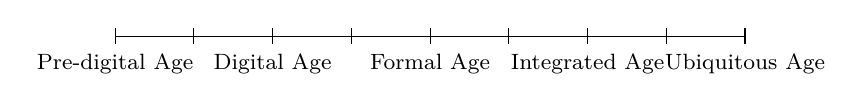
\begin{tikzpicture}
    \draw (0,0) -- (8,0);
    \foreach \x in {0,1,...,8} {
      \draw (\x,-0.1) -- (\x,0.1);
    }
    \foreach \x/\y in {0/Pre-digital Age, 2/Digital Age, 4/Formal Age, 6/Integrated Age, 8/Ubiquitous Age} {
      \node[anchor=north] at (\x,-0.1) {\footnotesize\y};
    }
  \end{tikzpicture}
  \caption{
    Timeline of the ages of data collection.
  }
  \label{fig:collection-history}
\end{figure}

\Cref{fig:collection-history} illutrates the timeline.

\subsubsection{Pre-digital age}

We can consider the earliest records of data collection to be the notches on sticks and
bones to keep tracking of passing of time.  The Lebombo bone, a baboon fibula with
notches, is probably the earliest known mathematical object.  It was found in the Lebombo
Mountains located between South Africa and Eswatini.
They estimate it is more
than 40,000 years old. It is conjectured to be a tally stick, but its exact purpose is
unknown. Its 29 notches suggests that may have been used as a lunar phase counter.
However, since it is broken at one end, the 29 notches may or may not be the total
number\footcite{Beaumont2013}.

Since the early forms of writing, humanity abilities to record events and information
increased significantly.  The first known written records date back to 3,500 BC, the
Sumerian archaic (pre-cuneiform) writing.  This writing system was used to represent
commodities using clay tokens and to record transactions\footcite{Ifrah1998}.

Another important milestone in the history of data collection is the record of
demographic data.  One of first known census was conducted in 3,800 BC in the Babylonian
Empire.  It was ordered to assess the population and resources of
his empire\footcite{Grajalez2013}.

Moving forward many years, I consider a major influential figure in the history of data
collection to be Florence Nightingale (1820 -- 1910).  She was a passionate statistician
and probably the first person to use statistics to influence public and official
opinion.  The meticulous records she kept during the Crimean War
(1853 -- 1856) were the evidence that saved lives.  She was also the first to use
statistical graphics to present data in a way that was easy to understand.  She is
credited with developing a form of the pie chart now known as the polar area
diagram.  She also reformed healthcare in the United Kingdom and
is considered the founder of modern nursing\footcite{Grajalez2013}.

\begin{mainbox}{Florence Nightingale}
  \begin{itemize}
    \item Passionate statistician.
    \item First person to use statistics to influence public and official opinion.
    \item Organized data from garden fruits and vegetables into numerical tables at the age of 9.
    \item At 20 she was receiving two-hour lessons from a Cambridge-trained mathematician.
    \item She found the sight of a long column of figures “perfectly reviving”.
    \item She went out to the Crimean War, to Scutari in Turkey, in 1854.
    \item She found that not even the numbers of soldiers entering the hospitals, or leaving them – alive or dead – was known.
    \item From the first she kept meticulous records.
    \item The data she collected was the evidence that saved lives.
    \item She was the first to use statistical graphics to present data in a way that was easy to understand.
    \item She is credited with developing a form of the pie chart now known as the polar area diagram.
    \item She reformed healthcare in the United Kingdom and is considered the founder of modern nursing.
  \end{itemize}
\end{mainbox}

\subsection{Timeline of data analysis}

\begin{itemize}
  \item Summary statistics
  \item Probability Advent 17, 18th
  \item Statistical learning 19th
    \begin{itemize}
      \item Bayes rule
      \item Gauss’ method of least squares
      \item Playfair data visualization
    \end{itemize}
  \item 20th inference
    \begin{itemize}
      \item Pearson hypothesis testing
      \item Fisher multivariate analysis, maximum likelihood estimate
    \end{itemize}
  \item Computer: McCulloch Pitts, Shannon information theory, Fix and Hodged discriminatory analysis, knn
  \item Machine learning: 1965 Nils Nilsson neural network, 1966 Hunt inducing trees, Kmeans, Vapnik 71
  \item Today: Ensembles, Deep learning: vision and language, KDD
\end{itemize}

\chapter{Fundamental concepts}
\label{chap:fundamental}
\glsresetall

\chapterprecishere{The simple believes everything,
  \par\raggedleft but the prudent gives thought to his steps.
  \par\raggedleft--- \textup{Proverbs 14:15} (ESV)}

A useful start point for someone studying data science is a definition of the term itself.
In this chapter, I discuss some definitions in literature and provide a definition of my
own.  As discussed in \cref{chap:history}, there is no consensus on the definition of data
science.  However, they all agree that data science is cross-disciplinary and a very
important field of study.

Another important discussion is the evidence that data science is actually a new science.
I argue that a ``new science'' is not a subject that its basis is built from the ground
up\footnote{As it would as unproductive as creating a ``new math'' for each new
application.  All ``sciences'' rely on each other in some way}, but a subject that has a
particular object of study and that meets some criteria.

Once we establish that data science is a new science, we need to understand one core
concept: data.  In this book, I focus on structured data, which are data that are organized
in a tabular format.  I discuss the importance of understanding the nature of the data we
are working with and how we represent them.

Finally, I discuss two important concepts in data science: database normalization and tidy
data.  Database normalization is mainly focused on the data storage.  Tidy data is mainly
focused on the requirements of data for analysis.  Both concepts interact with each other
and have their mathematical foundations.  I bridge the gap between the two concepts by
discussing their common mathematical foundations.

\begin{mainbox}{Chapter remarks}

  \boxsubtitle{Contents}

  \startcontents[chapters]
  \printcontents[chapters]{}{1}{}
  \vspace{1em}

  \boxsubtitle{Context}

  \begin{itemize}
    \itemsep0em
    \item There is no consensus on the definition of data science.
    \item Understanding the nature of data is important to extract knowledge from them.
    \item Structured data are data that are organized in a tabular format.
  \end{itemize}

  \boxsubtitle{Objectives}

  \begin{itemize}
    \itemsep0em
    \item Define data science.
    \item Present the main concepts about data theory.
  \end{itemize}

  \boxsubtitle{Takeaways}

  \begin{itemize}
    \itemsep0em
    \item Data science is a new science that studies the knowledge extraction from
      measurable phenomena using computational methods.
    \item Database normalization and tidy data are complementary concepts that interact
      with each other.
  \end{itemize}
\end{mainbox}

{}
\clearpage

\section{Data science definition}

In literature, we can find many definitions and descriptions of data science.

For \textcite{Zumel2019}\footfullcite{Zumel2019}, \emph{``data science is a cross-disciplinary practice that draws
on methods from data engineering, descriptive statistics, data mining, machine learning,
and predictive analytics.''}  They compare the area with the operations research, stating
that data science focuses on implementing data-driven decisions and managing their
consequences.

\textcite{Wickham2023}\footfullcite{Wickham2023} state that \emph{``data science is an exciting discipline that
allows you to transform raw data into understanding, insight, and knowledge.''}

\textcite{Hayashi1998}\footfullcite{Hayashi1998} says that data science ``is not only a
synthetic concept to unify statistics, data analysis and their related methods, but also
comprises its results'' and that it ``intends to analyze and understand actual phenomena
with `data.'{}''

I find the first definition too restrictive once new methods and techniques are always
under development.  We never know when new ``data-related'' methods will become obsolete
or a trend.  Also, \citeauthor{Zumel2019}'s view gives the impression that data science is a
operations research subfield.  Although I do not try to prove otherwise, I think it
is much more useful to see it as an independent field of study.  Obviously, there are
many intersections between both areas (and many other areas as well).  Because of such
intersections, I try my best to keep definitions and
terms standardized throughout chapters, sometimes avoiding popular terms that may generate
ambiguities or confusion.

The second one is not really a definition.  However, it states clearly \emph{what} data
science enables us to do.  The terms ``understanding,'' ``insight,'' and ``knowledge'' are
very important in the context of data science.  They are the goals of a data science
project.

The third definition brings an important aspect behind the data: the phenomena from which
they come.  Data science is not only about data, but about understanding the phenomena
they represent.

Note that these definitions do not contradict each other.  But, they do not attempt to
emphasize the ``science'' aspect of it.  From these thoughts, let us define the term.

\begin{defbox}{Data science}{ds}
  Data science is the study of knowledge extraction from
  measurable phenomena using computational methods.
\end{defbox}

I want to highlight the meaning of some terms in this definition.  \emph{Computational methods} means
that data science methods use computers to handle data and perform the calculations.
\emph{Knowledge} means information that humans can easily understand and/or apply to solve
problems.  \emph{Measurable phenomena} are events or processes where raw data can be
quantified in some way\footnote{%
  Non-measurable phenomena are related to metaphysics and are not the object of study in
  data science.  They are be the object of study in other sciences, such as
  philosophy, theology, etc.  However, many metaphysics concepts are borrowed to
  explain data science concepts.%
}.  \emph{Raw data} are data collected directly from some source and
that have not been subject to any other transformation by a software program or a human
expert.  \emph{Data} is any piece of information that can be digitally stored.


\textcite{Kelleher2018} summarize very well the challenges data science takes up:
``extracting non-obvious and useful patterns from large data sets [\dots]; capturing,
cleaning, and transforming [\dots] data; [storing and processing] big [\dots] data sets;
and questions related to data ethics and regulation.''

Data science naming contrasts with conventional sciences.  Usually, a ``science'' is named after
its object of study.  Biology is the study of the life, Earth science studies the planet
Earth, and so on.  I argue that data science does not study data itself, but how we can
use them to understand a certain phenomenon.

One similar example is ``computer science.''  Computer science is not the study of
computers themselves, but the study of computing and computer systems.  Similarly, one
could state that data science studies knowledge extraction\footnote{Related to data
analysis, see \cref{sub:time-analysis}.} and data systems\footnote{Related to data
handling, see \cref{sub:time-handling}.}.

Moreover, the conventional scientific paradigm is
essentially model-driven: we observe a phenomenon related to the object of study, we
reason the possible explanation (the model or hypothesis), and we validate our hypothesis
(most of the time using data, though).  In data science, however, we extract the knowledge
directly and primarily from the data.  The expert knowledge and reasoning may be taken
into account, but we give data the opportunity to surprise us.

Thus, while the objects of the study in conventional sciences are the phenomena themselves
and the models that can explain them, the objects of the study in data
science are the means (computational methods and processes) that can extract reliable and ethical
knowledge from data acquired from any measurable phenomenon --- and, of course, their
consequences.

\def\verrids{(0,0) circle (20mm)}
\def\verrist{(-2.5,0) circle (15mm)}
\def\verride {(2.5,0) circle (15mm)}
\def\verrics {(0,-2.5) circle (15mm)}

\begin{figurebox}[label=fig:myview]{My view of data science.}
  \centering
  \begin{tikzpicture}
    \begin{scope}
      \clip \verrids;
      \fill[filled] \verrist;
      \fill[filled] \verride;
      \fill[filled] \verrics;
    \end{scope}
    \draw[outline] \verrids node(ds) {};
    \draw[outline] \verrist node {Statistics};
    \draw[outline, text width=27mm, text centered] \verride node {Philosophy / domain expertise};
    \draw[outline] \verrics node {Computer science};
    \node[anchor=north,above] at (0, 1) {Data science};
  \end{tikzpicture}
  \tcblower
    Data science is an entire new science.  Being a new science
    does not mean that its basis is built from the ground up.  Most of the subjects in
    data science come from other sciences, but its object of study (computational methods
    to extract knowledge from measurable phenomena) is particular enough to unfold
    new scientific questions -- such as data ethics, data collection, etc.
    Note that I emphasize philosophy over domain expertise because, in terms
    of scientific knowledge, the former is more general than the latter.
\end{figurebox}

\Cref{fig:myview} shows my view of data science.  Data science is an entire new science
that incorporates concepts from other sciences.  In the next section, I argue the reasons
to understand data science as a new science.

\section{The data science continuum}

In the previous section, I argued that data science is a new science defining its object
of study.  This is just the first step to establish a new science, especially because the
object of study in data science is not new.  Computer science, statistics, and other
sciences have been studying methods to process data for a long time.

One key aspect of the establishment of a new science is the social demand and the
importance of the object of study in our society.  Many say that ``data is the new oil.''
This is because the generation, storage and processing of data has increased exponentially
in the last decades.  As a consequence, whoever holds the data and can effectively extract
knowledge from them has a competitive advantage.

As a consequence of the demand, a set of methods are developed and then experiments are
designed to assess their effectiveness.  If the methods are effective, they gain
credibility, are widely accepted, and become the foundation of a new scientific
discipline.

Usually, a practical consequence of academic recognition is the creation of a new courses
and programs in universities.  This is the case of data science.  Many universities have
created data science programs in the last years.

Once efforts to develop the subject increase, it is natural that methodologies evolve and
that questions not particularly related to any other science.  This effect produces what I
call the ``data science continuum.''

In a continuum, the subject is not a new science yet.  It is a set of methods and
techniques borrowed from other sciences.  However, some principles emerge that are
connected with more than one already established science.  (For instance, a traditional
computational method adapted to assume statistical properties of the data.)  With time,
the premises and hypothesis of new methods become distinctive.  The particular properties
of the methods lead to the inception of methodologies to validate them. While validating
the methods, new questions arise.

\begin{figurebox}[label=fig:continuum]{The data science continuum.}
  \centering
  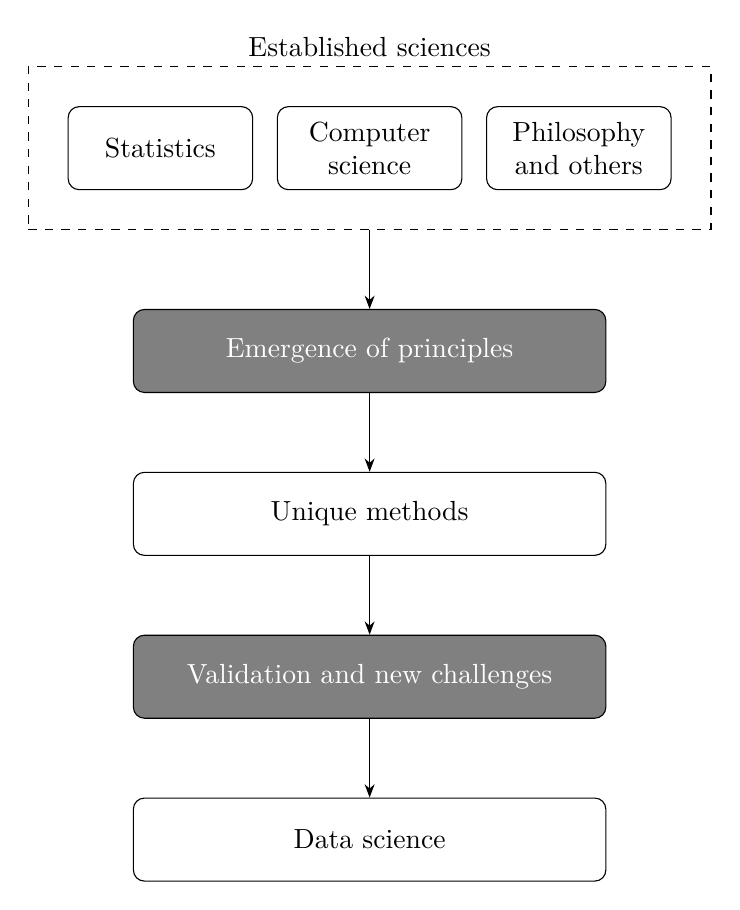
\begin{tikzpicture}[node distance=10mm and 3mm]
    % Base Layer: Established Sciences
    \node (stats) [block] {Statistics};
    \node (cs) [block, right=of stats] {Computer science};
    \node (ds) [block, right=of cs] {Philosophy and others};
    % A box around the Base Layer
    \node (basebox) [draw, dashed, inner sep=0.5cm, fit={(stats) (ds)}, label=above:{Established sciences}] {};
    % Middle Layer: Emergence of Principles
    \node (principles) [darkblock, below=of basebox, minimum width=6cm, text width=5cm] {Emergence of principles};
    % Top Layer: Unique Methods and Validation
    \node (methods) [block, below=of principles, minimum width=6cm, text width=5cm] {Unique methods};
    \node (validation) [darkblock, below=of methods, minimum width=6cm, text width=5cm] {Validation and new challenges};
    \node (science) [block, below=of validation, minimum width=6cm, text width=5cm] {Data science};
    % Arrows
    \draw[-{Stealth}] (basebox) -- (principles);
    \draw[-{Stealth}] (principles) -- (methods);
    \draw[-{Stealth}] (methods) -- (validation);
    \draw[-{Stealth}] (validation) -- (science);
  \end{tikzpicture}
  \tcblower
    The data science continuum is the process of development of data science as a new
    science.  It began by borrowing methods and techniques from established sciences. Over
    time, distinct principles emerged that spanned multiple disciplines. As these
    principles developed, new methods and their premises became unique. This uniqueness
    led to the creation of specific methodologies for validating these methods. During the
    validation process, new questions and challenges arose, further distinguishing data
    science from its parent disciplines.
\end{figurebox}

The data science continuum is an instance of this process; see \cref{fig:continuum}.  At
first glance, data science seems like just a combination of computer science, statistics,
linear algebra, etc. However, the principles and priorities of data science are not the
same as the ones in that disciplines.  Similarly, the accepted methodologies in data
science differ, and keep evolving, from the ones in the other sciences.  New questions
like arise such as:
\begin{itemize}
  \itemsep0em
  \item How can we guarantee that the data we are using are reliable?
  \item How can we collect data in a way that does not bias our conclusions?
  \item How can we guarantee that the data we are using are ethical?
  \item How can we present our results in a way that is understandable to non-experts?
\end{itemize}

\section{Fundamental data theory}

As I stated, data science is not a isolated science.  It incorporates several concepts
from other fields and sciences.  In this section, I explain the basis of each component of
\cref{def:ds}.

\subsection{Phenomena}
\label{sub:phenomena}

Phenomenon is a term used to describe any observable event or process.  They are the
source we use to understand the world around us.  In general, we use our senses to
perceive phenomena.  To make sense of them, we use our knowledge and reasoning.

Philosophy is the study of knowledge and reasoning.  It is a very broad field of study
that has been divided into many subfields.  One possible starting point is \gls{ontology},
which is the study of being, existence, and reality.  Ontology studies what exists and how
we can classify it.  In particular, ontology describes the nature of categories,
properties, and relations.

Aristotle (384 -- 322 BC) is one of the first philosophers to study ontology. In
Κατηγορίαι\footnote{For Portuguese readers, I suggest \fullcite{CategoriesUnesp}.}, he
proposed a classification of the world into ten categories. Substance, or οὐσία,
is the most important one.  It is the category of being.  The other categories
are properties, quantity, quality, relation, place, time, position, state, and action.

Although rudimentary\footnote{Most historians agree that Categories was written before
Aristotle's other works.  Many concepts are further developed in his later works.},
Aristotle's categories served as a basis for the development of logical reasoning and
scientific classification, especially in the Western world.  The categories are still
still used in many applications, including computer systems and data systems.

Aristotle marked a rupture with many previous philosophers.  While Heraclitus (\nth{6}
century -- \nth{5} century BC) defended that everything is in a constant state of flux and
Plato (c. 427 -- 348 BC) defended that only the perfect can be known, Aristotle focused in
the world we can perceive and understand.  His practical view also opposed Antisthenes (c.
446 -- 366 BC) view that the predicate determines the object, which leads to the
impossibility of negation and consequently contradiction.

What is the importance of ontology for data science?  Describing, which is basically
reducing the complexity of the world to simple, small pieces, is the first step to
understand any phenomenon.  Drawing a simplistic parallel, phenomena are like the
substance category, and the data we collect are like the other categories, which describe
the properties, relations, and states of the substance.  A person that can easily organize
their thoughts to identify the entities and their properties in a problem is more likely
to collect relevant data.  Also, the understanding of logical and grammatical limitations
--- such as univocal and equivocal terms --- is important to avoid errors in data
science applications\footnote{It is very common to see data scientists reducing the
meaning of the columns in a dataset to a single word.  Or even worse, the assume
that the same word in different columns have the same meaning.  This is a common source
of errors in data science projects.}.

Another important field in Philosophy is epistemology, which is the study of knowledge.
Epistemology elaborates on how we can acquire knowledge and how we can distinguish between
knowledge and opinion.  In particular, epistemology studies the nature of knowledge,
justification, and the rationality of belief.

Finally, logic is the study of reasoning.  It studies the nature of reasoning and
argumentation.  In particular, logic studies the nature of inference, validity, and
fallacies.

I further discuss knowledge and reasoning in \cref{sub:knowledge}.

In the context of a data science project, we usually focus on phenomena from particular domain of
expertise.  For example, we may be interested in a phenomena related to the stock
market, or related to the weather, or related to the human
health.  Thus, we need to understand the nature of the phenomena we are studying.

Fully understanding the phenomena we are tackling requires both a general knowledge
of epistemology, ontology, and logic, and a particular knowledge of the domain of
expertise.

Observe as well that we do not restrict ourselves to the intellectual understanding of
philosophy.  There are several computational methods that implements the concepts of
epistemology, ontology, and logic.  For example, we can use a computer to perform
deductive reasoning, to classify objects, or to validate an argument.  Also, we have
strong mathematical foundations and computational tools to organize categories, relations, and
properties.

The reason we need to understand the nature of the phenomena we are studying is that we
need to guarantee that the data we are collecting are relevant to the problem we are
trying to solve.  Incorrectly perception of the phenomena may lead to incorrect data
collection, which certainly lead to incorrect conclusions.

\subsection{Measurements}

Similarly to Aristotle's work, data scientists focus on the world we can perceive with our
senses (or using external sensors).  In a more restrictive way, we focus on the world we
can measure\footnote{Some phenomena might be knowable but not measurable.  For example,
the existence of God is a knowable phenomenon, but it is not measurable.}. Measurable
phenomena are
those that we can quantify in some way.  For example, the temperature of a room is a
measurable phenomenon because we can measure it using a thermometer.  The number of
people in a room is also a measurable phenomenon because we can count them.

When we quantify a phenomenon, we perform data collection.  Data collection is the process
of gathering data on targeted phenomenon in an established systematic way.
Systematic means that we have a plan to collect the data and we understand the
consequences of the plan, including the sampling bias.  Sampling bias is the influence
that the method of collecting the data has on the conclusions we can draw from them.
Once we have collected the data, we need to store them.  Data storage is the process of
storing data in a computer.

To perform those tasks, we need to understand the nature of data.  Data are any piece of
information that can be digitally stored.  Data can be stored in many different formats.
For example, we can store data in a spreadsheet, in a database, or in a text file.  We can
also store data in many different types.  For example, we can store data as numbers,
strings, or dates.

In data science, studying data types is important because they need to correctly reflect
the nature of the source phenomenon and be compatible with the computational methods we
are using.  Data types also restrict the operations we can perform on the data.

The foundation and tools to understand data types come from computer science.  Among the
subfields, I highlight:
\begin{itemize}
  \itemsep0em
  \item Algorithms and data structures: the study of data types and the computational
    methods to manipulate them.
  \item Databases: the study of storing and retrieving data.
\end{itemize}

The basic concepts are the same independently of the programming language, hardware
architecture, or the \gls{rdbms} we are using.  As a consequence, in this book, I focus on
the concepts and not on the tools.

\subsection{Knowledge extraction}
\label{sub:knowledge}

Like discussed before, knowledge and reasoning are important aspects of data science.
Philosophical and mathematical foundations from epistemology and logic provide us ways
to obtain knowledge from a set of premises and known (and accepted) facts\footnote{In
mathematics, we call the premises and accepted facts as axioms.  Corollaries,
lemmas, and theorems are the results of the reasoning process.}.

Deductive reasoning is the process of deriving a conclusion (or new knowledge) from
a set of previous knowledge.  Deductive reasoning, thus, enables us to infer
generalization rules from generalization rules.

Important figures that bridged the gap between philosophy and mathematics are
René Descartes (1596 -- 1650) and Gottfried Wilhelm Leibniz (1646 -- 1716).  Descartes
was the first to use algebra to solve knowledge problems, effectively creating
methods to mechanize reasoning.  Leibniz, after Descartes, envisioned a universal
algebraic language that would encompass logical principles and methods. Their work
influenced the development of calculus, Boolean algebra, and many other fields.

Once we have collected and stored the data, we need to extract knowledge from them.
Knowledge extraction is the process of obtaining knowledge from data.  The reasoning
principle here is inductive reasoning.  Inductive reasoning is the process of deriving
generalization rules from specific observations.  Inductive reasoning and data analysis
are closely related.  Refer to \cref{sub:time-analysis} for a timeline of the development
of data analysis.

In data science, we use computational methods to extract knowledge from data.  These
computational methods may come from many different fields.  In particular, I highlight:
\begin{itemize}
  \itemsep0em
  \item Statistics: the study of data collection, organization, analysis, interpretation,
    and presentation.
  \item Machine learning: the study of computational methods that can automatically learn from data.
    It is a branch of artificial intelligence.
  \item Operations research: the study of computational methods to optimize decisions.
\end{itemize}

Also, many other fields contribute to the development of domain-specific computational
methods to extract knowledge from data.  For example, in the field of biology, we have
bioinformatics, which is the study of computational methods to analyze biological data.
Earth sciences have geoinformatics, which is the study of computational methods to
analyze geographical data.  And so on.

Each method has its own assumptions and limitations.  Thus, we need to understand the
nature of the methods we are using.  In particular, we need to understand the
expected input and output of them.  Whenever the available data do not match the
requirements of the method, we may perform data preprocessing\footnote{%
  It is important to highlight that it is expected that some of the methods assumptions
  are not fully met.  These methods are usually robust enough to extract valuable
  knowledge even when data contain imperfections, errors and noise.  However, it is still
  useful to perform data preprocessing to adjust data as much as possible.%
}.

Data preprocessing mainly includes data cleaning, data transformation, and data
enhancement. Data cleaning is the process of detecting and correcting (or removing)
corrupt or inaccurate pieces of data.  Data transformation is the process of converting
data from one format or type to another.  Data enhancement is the process of adding
additional information to the data, usually, by integrating
data from different sources into a single, unified view.

% vim: set spell spelllang=en:

\chapter{Data science project}

\chapterprecishere{Figured I could throw myself a pity party or go back to school and
learn the computers. \par\raggedleft--- \textup{Don Carlton}, Monsters University (2013)}

First of all, a data science project is a software project.  The difference between a data
science software and a traditional software is that some components of the former is
constructed from data.  This means that part of the solution cannot be designed from the
knowledge of the domain expert, but must be learned from the data.  (Alternatively, the
cost of designing the solution is too high, and it is more efficient to learn it from the data.)

One good example of a data science project is a spam filter.  The spam filter is a software
that classifies emails into two categories: spam and non-spam.  The software is trained
using a set of emails that are already classified as spam or non-spam.  The software is
then used to classify new emails.  The software is a data science software because the
classification algorithm is learned from the data, i.e. the filters are not designed ``by
hand''.

% TODO:
% - the need of methodologies for data science projects
% - CRISP-DM
% - Nina's approach
% - Agile
% - Problems and advantages of SCRUM
% - Our approach

\section{CRISP-DM}

CRISP-DM\footnote{Official guide available at
\url{https://www.ibm.com/docs/it/SS3RA7_18.3.0/pdf/ModelerCRISPDM.pdf}.} is a methodology
for data mining projects.  It is an acronym for Cross Industry Standard Process for Data
Mining.  It is a methodology that was developed in the 1990s by IBM, and it is still
widely used today.

CRISP-DM is a cyclic process.  The process is composed of six phases:
\begin{enumerate}
  \item Business understanding: this is the phase where the project objectives are
    defined.  The objectives must be defined in a way that is measurable.  The phase also
    includes the definition of the project plan.
  \item Data understanding: this is the phase where the data is collected and explored.
    The data is collected from the data sources, and it is explored to understand its
    characteristics.  The phase also includes the definition of the data quality
    requirements.
  \item Data preparation: this is the phase where the data is prepared for the modeling
    phase.  The data is cleaned, transformed, and aggregated.  The phase also includes the
    definition of the modeling requirements.
  \item Modeling: this is the phase where the model is trained and validated.  The model is
    trained using the prepared data, and it is validated using the validation data.  The
    phase also includes the definition of the evaluation requirements.
  \item Evaluation: this is the phase where the model is evaluated.  The model is evaluated
    using the evaluation data.  The phase also includes the definition of the deployment
    requirements.
  \item Deployment: this is the phase where the model is deployed.  The model is deployed
    using the deployment requirements.  The phase also includes the definition of the
    monitoring requirements.
\end{enumerate}

\Cref{fig:cripdm} shows a diagram of the CRISP-DM process.  Note that the process is
cyclic and completly focused on the data.  The process do not address the software
development aspects of the project.

\begin{figurebox}[label=fig:cripdm]{Diagram of the CRISP-DM process.}
  \centering
  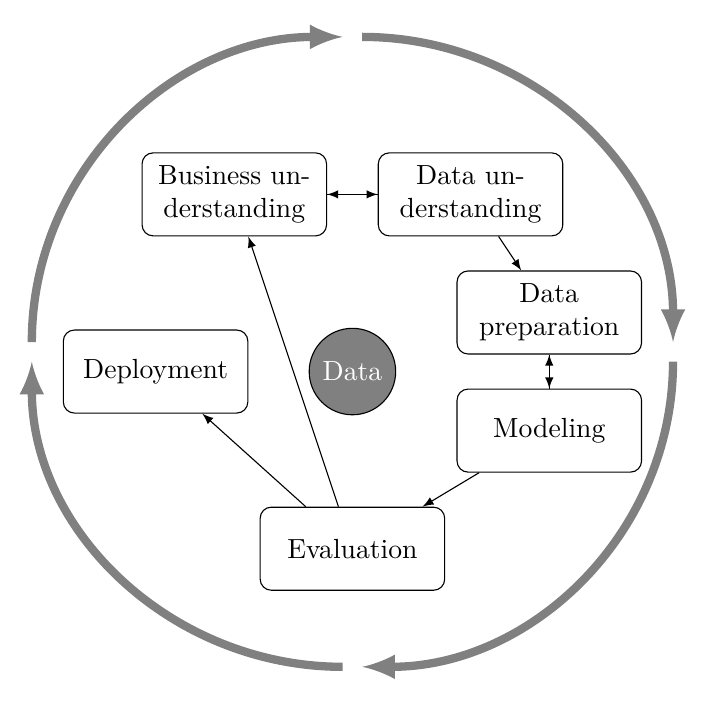
\begin{tikzpicture}[%
      block/.style={rectangle, draw, fill=white!20, text width=6em, text centered, rounded corners, minimum height=3em},
      line/.style={draw, -latex},
      bigarrow/.style={draw, -latex, line width=3pt, gray}
      ]
    \node (1) at (0, 0) {};
    \node (2) at (4, -4) {};
    \node (3) at (0, -8) {};
    \node (4) at (-4, -4) {};

    \node [block] (bu) at (-1.5, -2) {Business understanding};
    \node [block] (du) at (1.5, -2) {Data understanding};
    \path [line] (bu) -- (du);
    \path [line] (du) -- (bu);

    \node [block] (dp) at (2.5, -3.5) {Data preparation};
    \node [block] (m) at (2.5, -5) {Modeling};
    \path [line] (dp) -- (m);
    \path [line] (m) -- (dp);

    \path [line] (du) -- (dp);

    \node [block] (e) at (0, -6.5) {Evaluation};
    \node [block] (d) at (-2.5, -4.25) {Deployment};

    \path [line] (m) -- (e);
    \path [line] (e) -- (d);
    \path [line] (e) -- (bu);

    \node [draw, circle, fill=gray, text centered, text=white] at (0, -4.25) {Data};

    \path [bigarrow] (1.east) to[out=0, in=90] (2.60);
    \path [bigarrow] (2.-60) to[out=-90, in=0] (3.east);
    \path [bigarrow] (3.west) to[out=180, in=-90] (4.-120);
    \path [bigarrow] (4.120) to[out=90, in=180] (1.west);
  \end{tikzpicture}
  \tcblower
  Each block represents a phase of the CRISP-DM process.  Data is the central element of
  the process.  Arrows represent the transitions between the phases.
\end{figurebox}

The CRISP-DM methodology is a good starting point for data science projects.  However, it
does not mean that should be followed strictly.  The process is cyclic and flexible, and
adaptations are possible at any stage of the process.

\section{Nina and Zumel's approach}

\textcite{Zumel2019} propose a methodology for data science projects.

They define five roles:
\begin{itemize}
  \item Project sponsor: represents the business interests and champions the project;
  \item Client: represents the end users’ interests and is the domain expert;
  \item Data scientist: sets and executes the analytic strategy and communicates with the
    sponsor and the client;
  \item Data architect: manages data and data storage and sometimes manages data
    collection;
  \item Operations: manages infrastructure and deploys final project results.
\end{itemize}

\citeauthor{Zumel2019}'s model is similar to CRISP-DM, but emphasizes that back-and-forth
is possible at any stage of the process.

\section{Agile}

Agile is a methodology for software development.  It is an alternative to the waterfall
methodology.  The waterfall methodology is a sequential design where each phase
must be completed before the next phase can begin.

The four values of agile manifesto are:
\begin{itemize}
  \item Individuals and interactions over processes and tools;
  \item Working software over comprehensive documentation;
  \item Customer collaboration over contract negotiation;
  \item Responding to change over following a plan.
\end{itemize}

\section{SCRUM}

SCRUM is an agile framework for software development.  It is a process framework for
managing complex projects.  It is a lightweight process framework, which means that it
provides just enough guidance to be effective.

Many consider that SCRUM is not adequate for data science projects.  The main reason is
that SCRUM is designed for projects where the requirements are known in advance.  Also,
that data science projects have exploratory phases, which are not well supported by SCRUM.

I argue that this view is wrong.  SCRUM is a framework, and it is designed to be adapted to
the needs of the project.  SCRUM is not a rigid process.  In the following, I propose an
extension to SCRUM that makes it suitable for data science projects.

(In real-world, most developers do not have hacking-level skills.  They are not autonomous
enough to work without a plan.  This is especially true for ``data scientists'', who are
often not even developers.  SCRUM is a good compromise between the need for autonomy and
the need for a detailed plan.  Project methodology is needed to ensure that the project is
completed in time and within budget.)

\section{Our approach}

We propose an extension to SCRUM that makes it suitable for data science projects.  The
extension is based on the following observations:
\begin{itemize}
  \item Data science projects have exploratory phases;
  \item \dots
\end{itemize}

Two other values must be added to the agile manifesto:
\begin{itemize}
  \item Model confidence/understanding over model performance;
  \item Beware of interactive environments.
\end{itemize}

\subsection{The roles}

Combine SCRUM roles with the roles defined by \textcite{Zumel2019}.

\subsection{The principles of our approach}

\begin{enumerate}
  \item Modularize the solution. Usually, in four main modules: frontend, backend,
    dataset, and model search.  The frontend is the user interface.  The backend is the
    server-side code.  The dataset is the data that is used to train the model.  The model
    search is the code that searches for the best model.
  \item Version control everything.  This includes the code, the data, and the
    documentation. The most used tool for code version control is Git.  For datasets,
    extensions to Git exist, such as DVC\footnote{\url{https://dvc.org/}}.  One important aspect
    is to version control the model search code.  Interactive environments such as Jupyter
    notebooks are not suitable for this purpose.  They can be used to draft the code, but
    the final version must be version controlled.
  \item Continuous integration and continuous deployment.  This means that the code is
    automatically (or at least semi-automatically) tested and deployed.  The backend and
    frontend code is tested using unit tests.  The model search code is tested using
    validation methods such as cross-validation and Bayesian analysis on the discovered
    models.  Usually the model search code is very computationally intensive, and it is
    not feasible to run it on every commit.  Instead, it is run periodically, for example
    once a day.  If the clould infrastructure required to run the model search code is not
    available to automate validation and deploymen, at least make sure that the code is
    easily runnable.  This means that the code must be well documented, and that the
    required infrastructure must be well documented.  Also aggregate commands using a
    Makefile or a similar tool.  Pay attention on the dependences between dataset and the
    model training.  If the dataset changes significantly, not only the deployed model
    must be retrained, but the model search algorithm may need to be rethought.
  \item Reports as deliverables.  During sprints, the deliverables of data exploration are
    reports.
  \item Setup quantitative goals.  Do not fall on the trap of forever improving the model.
    Instead, setup quantitative goals for the model performance.  For example, the model
    must have a precision of at least 90\%.  Once you reach the goal, prioritize other
    tasks.
  \item Measure \emph{exactly} what you want.  During model validation, use your own
    metrics based on the project goals.  Usually, more than one metric is needed, and they
    might be conflicting.  Use strategies to balance the metrics, such as Pareto
    optimization.  Beware of the metrics that are most used in the literature.  They might not
    be suitable for your project.  Notice that during model training, some methods are
    limited to the loss functions that they can optimize.  If possible, choose a method
    that can optimize the loss function that you want.  Even if you are not explicitly
    optimizing the wanted metric, you might find a model that performs well on that metric.
    That is a reason validation is important.
  \item Report model stability and performance variance.  Understanding the limitations
    and characteristics of the model is more important than the model performance.  For
    example, if the model performance is high, but the model is unstable, it is not
    suitable for production.  Also, in some scenarios, interpretability is more important than
    performance.
  \item In user interface, mask data-science-specific terminology.  Usually, data science
    software gives the user the option to choose the model.  In order to avoid confusion,
    the user interface must mask the data-science-specific terminology.  This helps non
    experts to use the software consciously.
  \item Monitor model performance in production.  If possible setup feedback from the user
    interface.  Avoid automation of model releases because concept drift usually requires
    exploratory analysis.
  \item Use the appropriate backend.  REST API vs websocket.
\end{enumerate}

\input{structured}
\chapter{Data handling}
\label{chap:handling}

\chapterprecishere{%
  Tidy datasets are all alike, but every messy dataset is messy in its own way.
  \par\raggedleft--- \textup{Hadley Wickham}, Tidy Data}

% Important: avoid the term "data manipulation" as it has a negative connotation

Data handling is the process of adjusting data to make it suitable for analysis.
It involves three main tasks: data transformation, data cleaning, and data integration.

In this chapter, we consider that tables are rectangular data structures in which values
of the same column share the same properties (i.e. the same type, same restrictions, etc.)
and each column has a name.  Moreover, we assume that any value is possibly
\emph{missing}.

\section{Data handling operators}

In the literature and in software documentation, you will find a variety of terms used to
describe data handling operations\footnote{%
  The terminology ``data handling'' itself is not universal.  Some authors and libraries
  call it ``data manipulation'', ``data wrangling'', ``data shaping'', or ``data
  engineering''.  I use the term ``data handling'' to avoid confusion with the term ``data
  manipulation'' which has a negative connotation in some contexts.}. %
They often refer to the same or similar operations, but the terminology can be confusing.
In this section, I present a summary of these operations mostly based on
\textcite{Wickham2023} definitions\footnote{Which are called \emph{verbs}.}.

\begin{slidebox}{Data handling operators}{}
  \begin{itemize}
    \item Filtering rows;
    \item Selecting columns;
    \item Mutating columns;
    \item Aggregating rows;
    \item Binding datasets;
    \item Joining datasets;
    \item Pivoting (spreading) and unpivoting (gathering) datasets.
  \end{itemize}
\end{slidebox}

These operations are the building blocks of the data handling tasks we will discuss in the
next sections.  They can also be extensively parametrized and combined to create more
elaborate data handling pipelines.  For instance, most of them can use predicates to
define the groups, arrangements, or conditions under which they should be applied.

We use the following terminology to refer to the data handling parameters:
\begin{itemize}
  \item \textbf{Predicate}: a function that returns a logical value, used to filter
    rows/columns or to define the groups of rows/columns to be processed;
  \item \textbf{Aggregation function}: a function that returns a single value given a vector
    of values (in which, the order of the values may be important);
  \item \textbf{Window function}: a function that returns a vector of values given a vector
    of values in which, the order of the values is important;
  \item \textbf{Expression}: a function that returns a vector of values, used to create new
    columns or to modify existing ones.
\end{itemize}

\begin{slidebox}{Data handling pipelines}{}
  \begin{itemize}
    \item Data handling operations can be combined to create complex pipelines;
    \item Operators may be reversible;
    \item Operators are vectorized;
    \item They can be parametrized with predicates, aggregation functions, and expressions;
    \item They operate on datasets and return new datasets as output.
    \item They are declarative.
  \end{itemize}
\end{slidebox}

Operators are also vectorized, meaning that they can be applied to multiple columns or
rows at once.  This is a key feature of data handling operations, as it allows for
expressive and efficient data manipulation.

Many of them are also reversible, meaning that they can be undone.  This is important
because it allows for reproducibility and traceability of the data handling process.

They operate on a dataset (or more than one) given as input and return a new dataset as
output.  This is important because it allows for the creation of data handling pipelines,
where the output of one operation is the input of the next one.  Parameters like column
names, predicates, aggregation functions, and expressions can be passed to these operations to
customize their behavior.

Unlike traditional procedural programming, where conditional statements and loops are used
to manipulate data, data handling operations are declarative.  This means that they are
expressed in terms of what should be done, not how it should be done.  This is a powerful
abstraction that allows for the creation of complex pipelines with a few lines of code.

\subsection{Filtering rows}

Filtering is the process of selecting a subset of rows from a dataset based on a
predicate.  If more than a single predicate is used, they are combined using a logical
operator, such as \texttt{AND} or \texttt{OR}.

After filtering, the dataset will contain only the rows that satisfy the predicate.
Columns remain unchanged.  This operation is potentially irreversible, as the removed
rows are lost.

In the basic form, each row is treated independently.  For instance, the predicate
\texttt{age > 18} will select all rows where the value in the \texttt{age} column is
greater than 18.

However, if the predicate depends on a aggregation or window function, one must specify
the groups and/or the order of the rows.  For instance, the predicate \texttt{age >
mean(age) group by country} will select the rows where the value in the \texttt{age}
column is greater than the mean of the \texttt{age} for each \texttt{country}. Another
example is the predicate \texttt{cumsum(price) < 100 sort by date}, which selects the rows
that satisfy the condition that the cumulative sum of the \texttt{price} column is less
than 100 given the order of the rows defined by the \texttt{date} column.

The trivial group is the entire dataset, so it is usually not necessary to specify it
explicitly.  However, it is usually not sensible to not specify the order of the rows.

When dealing with real values, be aware of floating-point precision issues.  In other
words, do not use the equality operator to compare real numbers.  Most of libraries
provide operators to compare real numbers within a given tolerance.

\begin{mainbox}{Practical tips}
  \begin{itemize}
    \item Use filtering to remove rows that are not relevant to your analysis;
    \item Use predicates to define the conditions under which rows should be removed;
    \item When aggregation functions are needed to define the predicate, specify the groups and
      the order of the rows;
    \item Be aware of floating-point precision issues when comparing real numbers.
  \end{itemize}
\end{mainbox}

\subsection{Selecting columns}

Selecting is the process of choosing a subset of columns from a dataset.  The remaining
columns are discarded.  This operation is not reversible, as the discarded columns are
lost.  Rows remain unchanged.

There are two main ways to select columns: by name or by predicate.  The former is the
most common and is used to select a fixed set of columns.  The latter is used to select
columns that satisfy a given condition, i.e., the values in the columns are used to
determine which columns should be selected.

When selecting columns by name, one can use a list of column names or a regular
expression\footnote{Regular expressions are very general and powerful, but they are also
complex and error-prone.  An alternative is to use some form of hierarchical naming,
such as \texttt{type.column} to express groups of columns.}.
The latter is useful when the column names follow a pattern that reflects the semantics of
the columns.  For instance,
one can use the regular expression \texttt{col[0-9]+} to select all columns whose names
start with \texttt{col} followed by one or more digits.

When selecting columns by predicate, one can use a function that returns a logical value
to define the condition under which a column should be selected.  For instance, one can
use the predicate \texttt{isnumeric} to select all columns that contain numeric values.
Notice, however, that the predicate is applied to each column independently and returns a
single logical value for each column.

Like filtering, selecting predicates might contain aggregation functions.  Although it is
theorically possible to consider the order of the values in the columns, it is not common
to do so.  (Especially because one would need to assume that the rows are previously
sorted by some criterion.) Groups, however, never make sense in this context, once the
predicate is applied to each column independently.

Depending on the context, it may be useful to ``drop'' columns instead of selecting them.
This is the same as selecting all columns except the ones specified.  This is useful when
the number of columns to be dropped is small compared to the total number of columns.
Strictly speaking, we just need to negate the predicate or the regular expression used to
select the columns.

Finally, it is very common to find libraries and framework in which the order of the
columns is important.  As a result, columns can be selected by position as well.
I find this practice error-prone and I recommend avoiding it whenever possible.

\begin{mainbox}{Practical tips}
  \begin{itemize}
    \item Use selecting to remove columns that are not relevant to your analysis;
    \item Use column names or regular expressions (or hierarchical names) to select columns;
    \item Use predicates (many to one, with no aggregation functions) to define the conditions
      under which columns should be selected;
    \item Avoid depending on the order of the columns.
  \end{itemize}
\end{mainbox}

\subsection{Mutating columns}

Mutating is the process of creating new columns.  The operation is reversible, as the
original columns are kept.  The new columns are added to the dataset.

The values in the new column are determined by an expression.  The expression is a
function that returns a vector of values given the values in the other columns.  The
expression can be a simple function, such as \texttt{y = x + 1}, or a more complex
function, such as \texttt{y = ifelse(x > 0, 1, 0)}.  Here, \texttt{x} and \texttt{y} are
the names of an existing and the new column, respectively.

One may also use a aggregation and window function in the expression. This is particularly
useful when performing mutation considering a group.  In this case, the returned value is
repeated (aggregation function) for each row of the same group.  Like in filtering, the
more explicit you can be about order and groups, the better.

For example, the expression \texttt{y = cumsum(x) group by category sort by date} will
create a new column \texttt{y} with the cumulative sum of the \texttt{x} column for each
\texttt{category} given the order of the rows defined by the \texttt{date} column.

Sometimes, the same expression can be used to create multiple columns.  This is useful
when the new columns are related.  To do so, one first specifies the columns in the same way as
when selecting columns.  Then, one needs to specify a rule to name the new columns.
For instance, \texttt{x\_new = x + 1 across x matches \textasciicircum{}col[0-9]+\$}.

Practically speaking, mutation can overwrite existing columns.  This is useful when the
new column is a replacement for the old one.  Formally, overwriting is just a sequence of
mutation and selection operations.

\begin{mainbox}{Practical tips}
  \begin{itemize}
    \item Use mutating to create new columns that are relevant to your analysis;
    \item Use expressions to define the values of the new columns;
    \item Use aggregation and window functions in the expression to create new columns based on
      groups and order;
    \item Use the same expression to create multiple columns when the new columns are related.
  \end{itemize}
\end{mainbox}

\subsection{Aggregating rows}

We can aggregate the rows of a dataset to create a new dataset with fewer rows.    The
operation is not reversible, as the discarded rows are lost.  The columns are also lost,
only the new aggregate columns remain.

The values in the new columns are determined by an aggregation function.  Like filtering
and mutation, the aggregation function can be parametrized by specifying a group and/or an
order.

The resulting dataset will contain one row for each group.  The values in the new columns
are determined by the aggregation function applied to the values in the other columns.
All columns that define the groups are usually kept in the resulting dataset.  In this
case, as expected, values of such columns are equal for all rows in the same group.

For instance, the aggregation function \texttt{mean(x) group by category} will create a
new dataset with one row for each different value of \texttt{category} and a new column
with the mean of the \texttt{x} column for each group.

\begin{mainbox}{Practical tips}
  \begin{itemize}
    \item Use aggregation to summarize the data in a dataset;
    \item Use aggregation functions to define the values of the new columns;
    \item Use the group and order parameters to define the groups and the behavior of the
      aggregation function.
  \end{itemize}
\end{mainbox}

\subsection{Binding datasets}

One trivial, yet important, operation is to bind datasets.  This is the process of
combining two or more datasets into a single dataset.  The operation is reversible, as the
original datasets are kept.  The new dataset contains all the rows and columns of the
original datasets.

There are two ways to bind datasets: by rows or by columns.  The former is used to
combine datasets that have exactly the same columns but represent different parts of the
same dataset.  The latter is used to combine datasets that comprise the same observations
(rows) but captures different aspects of the same dataset.

When binding datasets by rows, the datasets must have the same columns\footnote{In
practice, it is usually required that they share the same order of the columns as well.
This is not a theoretical requirement, but a common limitation of most libraries.}.
The resulting dataset will contain all the rows of the original datasets.  The columns
remain unchanged.  It is a good practice to create a new column that represents the source
of each row.  For instance, if each table represents data collected in a different year,
one can create a new column \texttt{year} that contains the year of the data.

When binding datasets by columns, the datasets must have the same number of rows.  Each
matching row represent the same observation\footnote{Practically speaking, either the
order of the rows or a key column is used to match the rows of the datasets.  In both
situations, this is equivalent to a join operation by the row number or the key column;
assuming that both datasets contains the same observations.}. The resulting dataset will
contain all the columns of the original datasets.  The rows remain unchanged.

\begin{mainbox}{Practical tips}
  \begin{itemize}
    \item Use binding to combine datasets that represent different parts of the same dataset;
    \item Use binding by rows to combine datasets that have the same columns --- in this
      case, create a new column that represents the source of each row;
    \item Use binding by columns to combine datasets that have the same number of rows.
  \end{itemize}
\end{mainbox}

\subsection{Joining datasets}

Joining is the process of combining two datasets into a single dataset based on common
columns.  The operation may not be reversible, consult \cref{sec:normalization} for more
details.

The join of two tables is the operation that returns a new table with the columns of both
tables.  Let \texttt{U} be the common set of columns.  For each occurring value of
\texttt{U} in the first table, the operation will look for the same value in the second
table.  If it finds it, it will create a new row with the columns of both tables.  If it
does not find it, no row will be created.  This operation assumes that values in \texttt{U}
are unique in each table.

The variation described above is usually called natural or inner join.  Three other
variations are possible.
\begin{itemize}
  \item Left join: for each occurring value of \texttt{U} in the first table, the operation
    will look for the same value in the second table.  If it finds it, it will create a new
    row with the columns of both tables.  If it does not find it, it will create a new row
    with the columns of the first table and missing values for the columns of the second
    table.
  \item Right join: the same as the left join, but the roles of the tables are reversed.
  \item Outer join: for each different value of \texttt{U} in both tables, the operation
    will create a new row with the columns of both tables.  If a value is missing in one
    table, it will be filled with a missing value.
\end{itemize}

\begin{mainbox}{Practical tips}
  \begin{itemize}
    \item Use joining to integrate datasets;
    \item Be aware of the risks of joining datasets (\cref{sec:normalization}), for
      example, that some joins may create invalid rows;
    \item Use the appropriate variation of the join operation in applications.
  \end{itemize}
\end{mainbox}

\subsection{Pivoting and unpivoting}

Another important operation is to pivot and unpivot datasets.  This is the process of
transforming a dataset from a long format to a wide format and vice versa.  The operations
is reversible and they are the inverse of each other.

Pivoting requires to specify a name column --- whose discrete and finite possible values
will become the names of the new columns --- and a value column --- whose values will be
spread across the rows.  All remaining columns are considered to be keys, uniquely
identifying each row of new the dataset.

Unpivoting\footnote{Which \citeauthor{Wickham2023} call pivot longer.} is the reverse
operation.  One must specify all the columns whose names are the values of the before
called name column.  The values of these columns will be gathered into a new column.
As before, all remaining columns are considered to be keys.

In practical applications, where not all remaining columns are keys, one must aggregate
rows beforehand.

\begin{tablebox}[label=tab:pivot]{Pivoting example.}
  \begin{minipage}{0.45\textwidth}
    \centering
    \rowcolors{2}{black!10!white}{}
    \begin{tabular}{ccc}
      \toprule
      \texttt{name} & \texttt{year} & \texttt{value} \\
      \midrule
      A & 2019 & 1 \\
      A & 2020 & 2 \\
      A & 2021 & 3 \\
      B & 2019 & 4 \\
      B & 2020 & 5 \\
      B & 2021 & 6 \\
      \bottomrule
    \end{tabular}
  \end{minipage}
  \hfill
  \begin{minipage}{0.45\textwidth}
    \centering
    \rowcolors{2}{black!10!white}{}
    \begin{tabular}{cccc}
      \toprule
      \texttt{name} & \texttt{2019} & \texttt{2020} & \texttt{2021} \\
      \midrule
      A & 1 & 2 & 3 \\
      B & 4 & 5 & 6 \\
      \bottomrule
    \end{tabular}
  \end{minipage}
  \tcblower
  The left table is in the long format and the right table is in the wide format.  The
  name column is \texttt{year} and the value column is \texttt{value}.
\end{tablebox}

\Cref{tab:pivot} shows an example of pivoting.  The left table is in the long format and
the right table is in the wide format.  The name column is \texttt{year}, the value column
is \texttt{value}, and the remaining column is \texttt{name} which is an unique identifier
of the rows in the wide format.

\begin{mainbox}{Practical tips}
  \begin{itemize}
    \item Use pivoting to transform datasets from a long format to a wide format;
    \item Use unpivoting to transform datasets from a wide format to a long format;
    \item Be aware of the need to aggregate rows before unpivoting.
  \end{itemize}
\end{mainbox}

\subsection{An algebra for statistical transformations}

In recent years, some researchers made an effort to create a formal algebra for
statistical transformations.  The idea is to create a set of operations that can be
combined to create complex statistical transformations.  This is similar to the idea of
relational algebra, which is a set of operations that can be combined to create complex
queries.

\textcite{Song2021}, for example, propose a formal paradigm for statistical data
transformation.  They present a data model, a algebra, and a formal language.  Their goal
is to create a standard for statistical data transformation that can be used by different
statistical software.

However, in my opinion, the major deficiency of their work is that they mostly try to
``reverse engineer'' the operations that are commonly used in statistical software.  This
is useful for the translation of code between different software, but it is not productive
to advance in the theoretical understanding of statistical transformations.

If one ought to tackle the challenge of formally expressing statistical transformations, I
think one should start from the basic operations.  Basic operations mean that they are
irreducible, i.e., they cannot be expressed as a sequence of other operations.

Some thoughts about it:
\begin{itemize}
  \item Binding columns can be expressed as a join operation, thus it is not a basic
    operation.
  \item Some software provide features that can be better expressed in other (often simpler) ways.  Row
    naming is an example.  It is useful to keep track of the origin of each row, but names
    can be just another column.  I argue for excluding row naming in a formal algebra.
  \item Some operations are very useful and recurring, even if they are not basic.  Such
    operations must be omitted from the formal algebra for the sake of simplicity.
    However, any software that implements a language for the formal algebra can provide
    syntax sugar for these operations.
  \item Not defining your algebra in terms of a specific programming language is a good
    practice.  This is because the algebra is a theoretical concept and should be
    independent of any implementation.  It also gives opportunities to rethink the
    things that commonly done in a specific way.  This can lead to new insights and
    correct error-prone practices.
  \item Pivoting seems to be ``different'' enough to the other operations to be considered
    in the set of basic operations.  However, it is not hard to see that they can be
    rewritten as joins with the meta tables containing the possible values of the
    attributes.
\end{itemize}

\section{Data transformation}

\subsection{Reshaping}

\subsection{Sampling}

\subsection{Dimensionality reduction}

\subsection{Normalization}

\begin{mainbox}{Practice!}
  Can you identify which data transformation operations are used to make datasets
  presented in \cref{chap:data} tidy?
\end{mainbox}

\section{Data cleaning}

\subsection{Missing data}

\subsection{Outliers}

\subsection{Noise}

\section{Data integration}

\subsection{Joining}

\subsection{Merging}

\subsection{Concatenating}

% vim: spell spelllang=en

% \input{exploratory} TODO
\chapter{Statistical learning theory}

\chapterprecishere{%
  To  understand  God's  thoughts  we  must study statistics, for these are the measure of His purpose.
  \par\raggedleft--- \textup{Florence Nightingale}, her diary}

We can address several kinds of problems using algorithms that learn from data.  However,
we focus on the problem of \emph{inductive learning}. Before we go further, let us define some terms.

\begin{defbox}{Artificial intelligence}{}
  The field that studies algorithms that exhibit intelligent behavior.
\end{defbox}

Artificial intelligence is a very broad field, including not only the study of algorithms
that exhibit intelligent behavior, but also the study of the behavior of intelligent
systems.  For instance, it encompasses the study of optimization methods, bioinspired algorithms,
robotics, philosophy of mind, and many other topics.  We are interested in the subfield of
artificial intelligence that studies algorithms that exhibit some form of intelligent
behavior.

\begin{defbox}{Machine learning}{}
  The subfield of artificial intelligence that studies algorithms that enable computers to
  automatically learn from data.
\end{defbox}

Machine learning is the subfield of artificial intelligence that studies algorithms that
enable computers to automatically learn and improve their performance on a task from
experience, without being explicitly programmed by a human being.

\begin{defbox}{Predictive learning}{}
  The machine learning paradigm that studies the problem of making predictions given known
  input data.
\end{defbox}

The machine learning paradigm that focuses on making predictions about outcomes (sometimes
about the future) based on historical data. Depending on the reasoning behind the learning
algorithms, the main predictive algorithms are classified in either inductive or
transductive.

\begin{defbox}{Inductive learning}{}
  The machine learning approach that involves deriving general rules from specific
  observations.
\end{defbox}

Induction a type of reasoning that goes from specific instances to more general
principles.  Inductive learning is the machine learning approach that studies algorithms
that, given data representing the set of specific instances, derive general rules that
can make predictions about \emph{any} new instances.

\Cref{fig:learning} give us a hierarchical view of the learning field.  Alternatives ---
such as descriptive learning in opposition to predictive learning, or transductive
learning in opposition to inductive learning --- are out of the scope of this course.

\begin{figurebox}[label=fig:learning]{Organizational chart of the learning field.}
  \centering
  \begin{tikzpicture}
    \draw[outline] (0,0) circle (30mm) node {};
    \node[below] at (0, 2.6) {artificial intelligence};
    \draw[outline] (0,-0.5) circle (25mm) node {};
    \node[below] at (0, 1.6) {machine learning};
    \draw[outline] (0,-1) circle (20mm) node {};
    \node[below] at (0, 0.5) {predictive learning};
    \draw[outline] (0,-1.5) circle (15mm) node {};
    \node[below] at (0, -1.0) {inductive learning};
  \end{tikzpicture}
  % \tcblower
  % Artificial intelligence is a very broad field, including not only the study of
  % algorithms that exhibit intelligent behavior, but also the study of the behavior of
  % intelligent systems.  Machine learning is a subfield of artificial intelligence that
  % studies algorithms that enable computers to automatically learn from data.  A particular
  % case of machine learning is predictive learning, which focuses on making predictions
  % about outcomes given known input data.  Inductive learning is a yet more specific type of
  % learning that involves deriving general rules from specific observations.
\end{figurebox}

Maybe the most general (and useful) framework for predictive learning is Statistical
Learning Theory.  In this chapter, we will introduce the basic concepts of this theory.

\section{Hypothesis}

Consider the set
\begin{equation}
  \label{eq:training-set}
  \big\{(\vec{x}_i, y_i) : i = 1, \dots, n \big\}
\end{equation}
where each sample $i$ is associated with a feature vector $\vec{x}_i \in \mathcal{X}$ and a target variable
$y_i \in \mathcal{Y}$.  We assume that samples are random independent identically
distributed (i.i.d.) observations drawn according to $$P(x, y) = P(x) P(y | x)\text{.}$$
Both $P(x)$ and $P(y|x)$ are fixed but unknown.

This is equivalent to the original learning problem stated by \textcite{Vapnik1995}, where
a generator produce random vectors $\vec{x}$ according to a fixed but unknown
probability distribution $P(x)$ and a supervisor returns an output value $y$ for every
input vector $x$ according to a conditional distribution function $P(y|x)$, also fixed but
unknown.

Moreover, note that this setup is compatible with the idea of tidy data and 3NF (see
\cref{sub:bridge}). Of course, we assume $X, Y$ are only the measured variables (or
non-prime attributes).  In practice, it means that we left aside the keys in the learning
process.

\section{The learning problem}

Consider a \emph{learning machine} capable of generating a set of functions $f(x;
\theta) \equiv f_\theta(x)$, $\theta \in \Theta$ and $f_\theta : \mathcal{X} \rightarrow \mathcal{Y}$.
The problem of learning is that of choosing, among all possible $f_\theta$, the one that
predicts the target variable the best possible way.

In order to learn, we must first define the \emph{loss} (or discrepancy) $\mathcal{L}$
between the response $y$ to a given input $x$, drawn from $P(x, y)$, and the
response provided by the learning machine.

Then, given the \emph{risk function}
\begin{equation}
  \label{eq:risk}
  R(\theta) = \int \mathcal{L}(y, f_\theta(x))\, dP(x, y)\text{,}
\end{equation}
the goal is to find the function $f_\theta$ that minimizes $R(\theta)$
where the only available information is the \emph{training set} \eqref{eq:training-set}.
This is the \emph{empirical risk minimization} (ERM) problem.

This formulation encompasses many specific problems. I focus on the two of them which I
believe are the most fundamental ones: \emph{binary data classification}\footnote{Vapnik
calls it \emph{pattern recognition}.} and \emph{regresssion estimation}\footnote{We are not talking about
\emph{regression analysis}.}.  I left aside the density estimation problem, once it is not
addressed in the remaining of the book.

\paragraph{Binary data classification task.}  In this task, the output $y$ take on
only two possible values, zero or one, and the functions $f_\theta$ are indicator
functions. For the loss
\begin{equation*}
  \mathcal{L}(y, f_\theta(x)) = \begin{cases}
    0 & \text{if } y = f_\theta(x) \\
    1 & \text{if } y \neq f_\theta(x)\text{,}
  \end{cases}
\end{equation*}
we aim at minimizing the risk $\eqref{eq:risk}$ which becomes the probability of
classification error.

\paragraph{Regression estimation task.} Let the outcome $y$ be a real value and
the \emph{regression} $r$ be $$r(x) = \int y\, dP(y|x) \text{.}$$

The regression function is the function $r = f_\theta$ that minimizes the risk function
\eqref{eq:risk} with the loss
\begin{equation*}
  \mathcal{L}(y, f_\theta(x)) = \big(y - f_\theta(x)\big)^2\text{.}
\end{equation*}

\section{ERM inductive principle}

In the following sections, $z$ describes the pair $(x, y)$ and $L(z, \theta)$ a generic loss
function.  The training dataset is thus a set of $n$ i.i.d. samples $z_1, \dots, z_n$.

Since the distribution $P(z)$ is unknown, the risk functional $R(\theta)$ is replaced by
the \emph{empirical risk functional}
\begin{equation}
  \label{eq:empirical-risk}
  R_n(\theta) = \frac{1}{n} \sum_{i=1}^n L(z_i, \theta)\text{.}
\end{equation}

Approximating $R(\theta)$ by the empirical risk functional $R_n(\theta)$ is the so called
ERM inductive principle.  The ERM principle is the basis of the statistical learning
theory.

Classical methods, such as least-squares, maximum likelihood, and maximum a posteriori are
all realizations of the ERM principle for specific loss functions and hypothesis spaces.

In the following sections, we address the four main questions of learning theory.  We
summarize them in \cref{tab:learning-questions}.

\begin{tablebox}[label=tab:learning-questions]{The four main questions of learning theory.}
  \begin{tabularx}{\textwidth}{@{}lX@{}}
    \toprule
    Part & Question \\
    \midrule
    \textbf{Consistency} &
      What are the necessary and sufficient conditions for consistency of a learning process? \\
    \textbf{Rate of convergence} &
      How fast is the rate of convergence of the learning process? \\
    \textbf{Generalization} &
      How can one controle the generalization ability of the learning process? \\
    \textbf{Construction} &
      How can one construct a learning machine that satisfies the conditions of consistency and generalization? \\
    \bottomrule
  \end{tabularx}
\end{tablebox}

\section{Consistency of learning processes}

\section{Rate of convergence of learning processes}

\section{Generalization ability of learning processes}

\section{Construction of learning machines}

\subsection{Data classification methods}

\subsection{Regression estimation methods}

\chapter{Data preprocessing}
\label{chap:preprocess}
\glsresetall

\chapterprecishere{I find your lack of faith disturbing.
  \par\raggedleft--- \textup{Darth Vader}, Star Wars: Episode IV -- A New Hope (1977)}

In this chapter, we discuss the data preprocessing, which is the process of adjusting the
data to make it suitable for a particular learning machine or, at the least, to ease the
learning process.

Similarly to data handling, data preprocessing is done by applying a series of operations
to the data.  However, some of the parameters of the operations are not fixed but rather
are fit from a data sampling.  In the context of inductive learning, the sampling is the
training set.

The operations are dependent on the chosen learning method.  So, when planning the
solution in our project, we must consider the preprocessing tasks that are necessary to
make the data suitable for the chosen methods.

I present the most common data preprocessing tasks in three categories: data cleaning,
data sampling, and data transformation.  For each task, I discuss the behavior of the data
preprocessing techniques in terms of fitting, adjustment of the training set, and
application of the preprocessor in production.

Finally, I discuss the importance of the default behavior of the model when the
preprocessing chain degenerates over a sample, i.e. when the preprocessor decides that it
has no strategy to adjust the data to make it suitable for the model.

\begin{mainbox}{Chapter remarks}

  \boxsubtitle{Contents}

  \startcontents[chapters]
  \printcontents[chapters]{}{1}{}
  \vspace{1em}

  \boxsubtitle{Context}

  \begin{itemize}
    \itemsep0em
    \item Tidy data is not necessarily suitable for modeling.
    \item Parameters of the preprocessor are fitted rather than fixed.
  \end{itemize}

  \boxsubtitle{Objectives}

  \begin{itemize}
    \itemsep0em
    \item Understand the main data preprocessing tasks and techniques.
    \item Learn the behavior of the preprocessing chain in terms of fitting, adjustment,
      and application.
  \end{itemize}

  \boxsubtitle{Takeaways}

  \begin{itemize}
    \itemsep0em
    \item Each learning method requires specific data preprocessing tasks.
    \item Fitting the preprocessor is crucial to avoid leakage.
    \item Default behavior of the model when the preprocessing chain degenerates must be
      specified.
  \end{itemize}
\end{mainbox}

{}
\clearpage

\section{Introduction}

In \cref{chap:data,chap:handling}, we discussed data semantics and the tools to
handle data.  They provide the grounds for preparation of the data as we described in the
data sprint tasks in \cref{sub:workflow}.  However, the focus is to guarantee that the
data is tidy and in the observational unit of interest, not to prepare it for modeling.

As a result, although data might be appropriate for the learning tasks we described in
\cref{chap:slt} --- in the sense that we know what the feature vectors and the target
variable are ---, they might not be suitable for the machine learning methods we will use.

One simple example is the perceptron (\cref{sub:perceptron}) that assumes that all
input variables are real numbers.  If the data contains categorical variables, we must
convert them to numerical variables before applying the perceptron.

For this reason, the solution sprint tasks in \cref{sub:workflow} include not only the
learning tasks but also the \emph{data preprocessing} tasks, which are dependent on the
chosen machine learning methods.

\begin{defbox}{Data preprocessing}{preprocessing}
  The process of adjusting the data to make it suitable for a particular learning machine
  or, at the least, to ease the learning process.
\end{defbox}

This is done by applying a series of operations to the data, like in data handling.  The
difference here is that some of the parameters of the operations are not fixed rather they
are fit from a data sampling.  Once fitted, the operations can be applied to
new data, sample by sample.

As a result, a data processing technique acts in three steps:
\begin{enumerate}
  \itemsep0em
  \item \textbf{Fitting}: The parameters of the operation are adjusted to the training
    data (which has already been integrated and tidied, represents well the phenomenon of
    interest, and each sample is in the correct observational unit);
  \item \textbf{Adjustment}: The training data is adjusted according to the fitted
    parameters, eventually, changing the sampling size and distribution;
  \item \textbf{Applying}: The operation is applied to new data, sample by sample.
\end{enumerate}

Understanding these steps and correctly defining the behavior of each of them is crucial
to avoid \gls{leakage} and to guarantee that the model will behave as expected in
production.

\subsection{Formal definition}
\label{sub:formal-preprocessing}

Let $T = (K, H, c)$ be a table that represents the data in the desired observational unit
--- as defined in \cref{sec:formal-structured-data}.  In this chapter, without loss of
generality --- as the keys are not used in the modeling process ---, we can consider $K =
\{1, 2, \dots\}$ such that $\rowcard[i] = 0$ if, and only if, $i > n$.  That means that
every row $r \in \{1, \dots, n\}$ is present in the table.

A data preprocessing strategy $F$ is a function that takes a table $T = (K, H, c)$ and
returns a adjusted table $T' = (K', H', c')$ and a fitted \emph{preprocessor} $f(z; \phi)
\equiv f_\phi(z)$ such that $$z \in \bigtimes_{h\, \in\, H} \domainof{h} \cup \{?\}$$ and $\phi$ are
the fitted parameters of the operation.  Similarly, $z' = f_\phi(z)$, called the
preprocessed tuple, satisfies $$z' \in \bigtimes_{h'\, \in\, H'} \domainof{h'} \cup
\{?\}\text{.}$$ Note that we make no restrictions on the number of rows in the adjusted
table, i.e., preprocessing techniques can change the number of rows in the training table.

In practice, strategy $F$ is a chain of dependent preprocessing operations $F_1$, \dots,
$F_m$ such that, given $T = T^{(0)}$, each operation $F_i$ is applied to the table
$T^{(i-1)}$ to obtain $T^{(i)}$ and the fitted preprocessor $f_{\phi_i}$.  Thus, $T' =
T^{(m)}$ and $$f(z; \phi = \{\phi_1, \dots, \phi_m\}) = \left(f_{\phi_1} \circ \dots \circ
f_{\phi_m}\right)(z)\text{,}$$ where $\circ$ is the composition operator.  I say that
they are dependent since none of the operations can be applied to the table without the
previous ones.

\subsection{Degeneration}

The objective of the fitted preprocessor is to adjust the data to make it suitable for the
model.  However, sometimes it can not achieve this goal for a particular input $z$.  This
can happen for many reasons, such as unexpected values, information ``too incomplete'' to
make a prediction, etc.

Formally, we say that the preprocessor $f_\phi$ degenerates over tuple $z$ if it outputs
$z' = f_\phi(z)$ such that $z' = (?, \dots, ?)$.  In practice, that means that the
preprocessor decided that it has no strategy to adjust the data to make it suitable for
the model.  For the sake of simplicity, if any step $f_{\phi_i}$ degenerates over
tuple $z^{(i)}$, the whole preprocessing chain degenerates\footnote{Usually, this is
implemented as an exception or similar programming mechanism.} over $z = z^{(0)}$.

Consequently, in the implementation of the solution, the developer must chose a default
behavior for the model when the preprocessing chain degenerates over a tuple.  It can
be as simple as returning a default value or as complex as redirecting the tuple to a
different pair of preprocessor and model.  Sometimes, the developer can choose to
integrate this as an error or warning in the user application.

\subsection{Data preprocessing tasks}

The most common data preprocessing tasks can be divided into three categories:
\begin{itemize}
  \itemsep0em
  \item Data cleaning;
  \item Data sampling; and
  \item Data transformation. % colocar enhancement aqui
\end{itemize}

In the next sections, I address some of the most common data preprocessing tasks
in each of these categories.  I present them at the order they are usually applied in the
preprocessing, but note that the order is not fixed and can be changed according to the
needs of the problem.

\section{Data cleaning}

Data cleaning is the process of removing errors and inconsistencies from the data.  This is
usually done to make the data more reliable for training and to avoid bias in the learning
process.  Usually, such errors and inconsistencies make the learning machines ``confused''
and can lead to poor performance models.

Also, it includes the process of dealing with missing information, which most machine
learning methods do not cope with.  Solutions range from the simple removal of the
observations with missing data to the creation of information to encode the missing data.

\subsection{Treating inconsistent data}

% TODO: move this somewhere when we talk about data handling and/or tidying
% Sometimes, during data collection, information is recorded using special codes.  For
% instance, the value 9999 might be used to indicate that the data is missing.  Such codes
% must be replaced with more appropriate values before modeling.  If a single variable
% encodes more than one concept, new variables must be created to represent each concept.

There are a few, but important, tasks to be done during data preprocessing in terms of
invalid and inconsistent data --- note that we assume that most of the issues in terms of
the semantics of the data have been solved in the data handling phase.  Especially in
production, the developer must be aware of the behavior of the model when it faces
information that is not supposed to be present in the data.

One of the tasks is to assert that physical quantities are dealt with standard units.  One must
check whether all columns that store physical quantities have the same unit of
measurement.  If not, one must convert the values to the same unit.  A summary of this
preprocessing task is presented in \cref{tab:unit-conversion}.

\begin{tablebox}[label=tab:unit-conversion]{Unit conversion preprocessing task.}
  \centering
  \rowcolors{2}{black!10!white}{}
  \begin{tabular}{lp{6cm}}
    \toprule
    \multicolumn{2}{c}{\textbf{Unit conversion}} \\
    \midrule
    % \textbf{Requirements} &
    %   A variable with the physical quantity and a variable with the unit of measurement. \\
    \textbf{Goal} &
      Convert physical quantities into the same unit of measurement. \\
    \textbf{Fitting} &
      None. User must declare the units to be used and, if appropriate, the conversion
      factors. \\
    \textbf{Adjustment} &
      Training set is adjusted sample by sample, independently. \\
    \textbf{Applying} &
      Preprocessor converts the numerical values and drop the unit of measurement column.  \\
    \bottomrule
  \end{tabular}
\end{tablebox}

Moreover, if one knows that a variable must follow a specific range of values, we can check
whether the values are within this range.  If not, one must replace the values with
missing data or with the closest valid value.  Alternatively, one can discard the
observation based on that criterion.  Consult \cref{tab:range-check} for a summary of this
operation.

\begin{tablebox}[label=tab:range-check]{Range check preprocessing task.}
  \centering
  \rowcolors{2}{black!10!white}{}
  \begin{tabular}{lp{6cm}}
    \toprule
    \multicolumn{2}{c}{\textbf{Range check}} \\
    \midrule
    % \textbf{Requirements} &
    %   A numerical variable. \\
    \textbf{Goal} &
      Check whether the values are within the expected range. \\
    \textbf{Fitting} &
      None. User must declare the valid range of values. \\
    \textbf{Adjustment} &
      Training set is adjusted sample by sample, independently.  If appropriate,
      degenerated samples are removed. \\
    \textbf{Applying} &
      Preprocessor checks whether the value $x$ of a variable are within the range $[a,
      b]$.  If not, it replaces $x$ with: (a) missing value $?$, (b) the closest valid
      value $\max(a, \min(b, x))$, or (c) degenerates (discards the observation). \\
    \bottomrule
  \end{tabular}
\end{tablebox}

Another common problem in inconsistent information is that the same category might be
represented by different strings.  This is usually done by creating a dictionary that maps
the different names to a single one, using standardizing lower or upper case, removing
special characters, or more advanced fuzzy matching techniques --- see
\cref{tab:text-standardization}.

\begin{tablebox}[label=tab:text-standardization]{Category standardization preprocessing task.}
  \centering
  \rowcolors{2}{black!10!white}{}
  \begin{tabular}{lp{6cm}}
    \toprule
    \multicolumn{2}{c}{\textbf{Category standardize}} \\
    \midrule
    % \textbf{Requirements} &
    %   A categorical variable. \\
    \textbf{Goal} &
      Create a dictionary and/or function to map different names to a single one. \\
    \textbf{Fitting} &
      None. User must declare the mapping. \\
    \textbf{Adjustment} &
      Training set is adjusted sample by sample, independently. \\
    \textbf{Applying} &
      Preprocessor replaces the categorical variables $x$ of a variable with the mapped
      value $f(x)$ that implements case standardization, special character removal, and/or
      dictionary fuzzy matching. \\
    \bottomrule
  \end{tabular}
\end{tablebox}

Note that these techniques parameters are not fitted from the data, but rather are fixed
from the problem definition.  As a result, they could be done in the data handling phase.
The reason we put them here is that the new data in production usually come with the
same issues.  Having the fixes programmed into the preprocessor makes it easier to
guarantee that the model will behave as expected in production.

\subsection{Outlier detection}

Outliers are observations that are significantly different from the other observations.
They can be caused by errors or by the presence of a different phenomena mixed in the data
collection process.  In both cases, it is important to deal with outliers before modeling.

The standard way to deal with outliers is to remove them from the dataset.  Assuming that
the errors or the out of distribution data appear randomly and rarely, this is a good
strategy.

Another approach is dealing with each variable independently.  This way, one can replace
the outlier value with missing data.  There are many ways to detect outlier values, but
the simplest one is probably a heuristic based on the \gls{iqr}.

Let $Q_1$ and $Q_3$ be the first and the third quartiles of the values in a variable,
respectively.  The \gls{iqr} is defined as $Q_3 - Q_1$.  The values that are less than
$Q_1 - 1.5\, \text{IQR}$ or greater than $Q_3 + 1.5\, \text{IQR}$ are considered outliers.
See \cref{tab:iqr-outlier}.

\begin{tablebox}[label=tab:iqr-outlier]{Outlier detection using the interquartile range.}
  \centering
  \rowcolors{2}{black!10!white}{}
  \begin{tabular}{lp{6cm}}
    \toprule
    \multicolumn{2}{c}{\textbf{Outlier detection using the IQR}} \\
    \midrule
    % \textbf{Requirements} &
    %   A numerical variable. \\
    \textbf{Goal} &
      Detect outliers using the IQR. \\
    \textbf{Fitting} &
      Store the values of $Q_1$ and $Q_3$ for each variable. \\
    \textbf{Adjustment} &
      Training set is adjusted sample by sample, independently. \\
    \textbf{Applying} &
      Preprocessor replaces the outlier values with missing data. \\
    \bottomrule
  \end{tabular}
\end{tablebox}

More sophisticated methods can be used to detect samples that are outliers, such as using
the definition of an outlier in the DBSCAN\footfullcite{Ester1996}. But, this is not
enough to fit the parameters of the preprocessor.  The reason is that descriptive methods
like DBSCAN  --- in this case, a method for clustering --- do not generalize to new data.
I suggest using methods like One-Class SVM\footfullcite{Scholkopf2001} to fit the
parameters of the preprocessor that detects outliers.  Thus, any new data point can
be classified as an outlier or not.

Like filtering operations in the pipeline, the developer must specify a default behavior
for the model when an outlier sample is detected in production.  See
\cref{tab:outlier-removal}.

\begin{tablebox}[label=tab:outlier-removal]{Task of filtering outliers.}
  \centering
  \rowcolors{2}{black!10!white}{}
  \begin{tabular}{lp{6cm}}
    \toprule
    \multicolumn{2}{c}{\textbf{Outlier removal}} \\
    \midrule
    % \textbf{Requirements} &
    %   A dataset with outliers. \\
    \textbf{Goal} &
      Remove the observations that are outliers. \\
    \textbf{Fitting} &
      Parameters of the outlier classifier. \\
    \textbf{Adjustment} &
      Training set is adjusted sample by sample, independently, removing
      degenerated samples. \\
    \textbf{Applying} &
      Preprocessor degenerates if the sample is classified as outliers and does
      nothing, otherwise. \\
    \bottomrule
  \end{tabular}
\end{tablebox}

\subsection{Treating missing data}

Since most models cannot handle missing data, it is crucial to deal with it in the data
preprocessing.

There are four main strategies to deal with missing data:
\begin{itemize}
  \itemsep0em
  \item Remove the observations (rows) with missing data;
  \item Remove the variables (columns) with missing data;
  \item Just impute the missing data;
  \item Use an indicator variable to mark the missing data and impute it.
\end{itemize}

Removing rows and columns are commonly used when the number of missing data is small
compared to the total number of rows or columns.  However, be aware that removing rows
``on demand'' can
artificially change data distribution, especially when the missing data is not missing at
random.  Row removal suffers from the same problem as any filtering operations
(degeneration) in the preprocessing step; the developer must specify a default behavior
for the model when a row is discarded in production.  See \cref{tab:row-removal-missing}.

\begin{tablebox}[label=tab:row-removal-missing]{Task of filtering rows based on missing data.}
  \centering
  \rowcolors{2}{black!10!white}{}
  \begin{tabular}{lp{6cm}}
    \toprule
    \multicolumn{2}{c}{\textbf{Row removal based on missing data}} \\
    \midrule
    % \textbf{Requirements} &
    %   A dataset with missing data. \\
    \textbf{Goal} &
      Remove the observations with missing data in any (or some) variables. \\
    \textbf{Fitting} &
      None. Variables to look for missing data are declared beforehand. \\
    \textbf{Adjustment} &
      Training set is adjusted sample by sample, independently, removing
      degenerated samples. \\
    \textbf{Applying} &
      Preprocessor degenerates over the rows with missing data in the specified variables.
      \\
    \bottomrule
  \end{tabular}
\end{tablebox}

In the case of column removal, the
preprocessor just learns to drop the columns that have missing data during fitting.
Beware that valuable information might be lost when removing columns for all the samples.

\begin{tablebox}[label=tab:col-drop-missing]{Task of dropping columns based on missing data.}
  \centering
  \rowcolors{2}{black!10!white}{}
  \begin{tabular}{lp{6cm}}
    \toprule
    \multicolumn{2}{c}{\textbf{Column removal based on missing data}} \\
    \midrule
    % \textbf{Requirements} &
    %   A dataset with missing data. \\
    \textbf{Goal} &
      Remove the variables with missing data. \\
    \textbf{Fitting} &
      All variables with missing data in the training set are marked to be removed. \\
    \textbf{Adjustment} &
      Columns marked are dropped from the training set. \\
    \textbf{Applying} &
      Preprocessor drops the chosen columns in fitting. \\
    \bottomrule
  \end{tabular}
\end{tablebox}

Imputing the missing data is usually done by replacing the missing values with some
statistic of the available values in the column, such as the mean, the median, or the
mode\footnote{More sophisticated methods can be used, such as the k-nearest neighbors
algorithm, for example, consult \fullcite{Troyanskaya2001}.}.  This is a simple and
effective strategy, but it can introduce bias in the data, especially when the number of
samples with missing data is large.  See \cref{tab:imputation}.

\begin{tablebox}[label=tab:imputation]{Task of imputing missing data.}
  \centering
  \rowcolors{2}{black!10!white}{}
  \begin{tabular}{lp{6cm}}
    \toprule
    \multicolumn{2}{c}{\textbf{Imputation of missing data}} \\
    \midrule
    % \textbf{Requirements} &
    %   A dataset with missing data. \\
    \textbf{Goal} &
      Replace the missing data with a statistic of the available values. \\
    \textbf{Fitting} &
      The statistic is calculated from the available data in the training set. \\
    \textbf{Adjustment} &
      Training set is adjusted sample by sample, independently. \\
    \textbf{Applying} &
      Preprocessor replaces the missing values with the chosen statistic. If an indicator
      variable is required, it is created and it is filled with the logical value:
      missing or not missing. \\
    \bottomrule
  \end{tabular}
\end{tablebox}

Just imputing data is not suitable when one is not sure whether the missing data is
missing because of a systematic error or phenomenon.  A model can learn the effect of the
underlying reason for missingness for the predictive task.
In that case, creating an indicator variable is a good strategy.  This is done by creating
a new column that contains a logical value indicating whether the data is missing or
not\footnote{Some kind of imputation is still needed, but we expect the model to deal
better with it since it can decide using both the indicator and the original variable.}.

Many times the indicator variable is already present in the data.  For instance, in a
dataset that contains information about pregnancy, let us say the number of days since
the last pregnancy.  This information certainly be missing if sex is male
or number of children is zero.  In this case, no new indicator variable is needed.
See \cref{tab:col-drop-missing}.

\section{Data sampling}

Once data is cleaned, the next step is (typically) to sample the data.  Sampling is the
process of selecting a random subset of the data or to create variations of the original
training set.

There are three main tasks that sample the data: subsampling, scope filtering and class
balancing.

\subsection{Random sampling}
\label{sub:random-sampling}

Some machine learning methods are computationally expensive and a smaller dataset might be
enough to solve the problem.  Random sampling is simply done by selecting a random subset
of the training data with a user defined size.

However, note that the preprocessor for this task \emph{must never do anything with the
new data} (or the test set we discuss in \cref{chap:planning}).  See
\cref{tab:random-sampling}.

\begin{tablebox}[label=tab:random-sampling]{Task of random sampling.}
  \centering
  \rowcolors{2}{black!10!white}{}
  \begin{tabular}{lp{6cm}}
    \toprule
    \multicolumn{2}{c}{\textbf{Random sampling}} \\
    \midrule
    % \textbf{Requirements} &
    %   A dataset with the scope of the phenomenon. \\
    \textbf{Goal} &
      Select a random subset of the training data. \\
    \textbf{Fitting} &
      None. User must declare the size of the sample. \\
    \textbf{Adjustment} &
      Rows of the training set are randomly chosen. \\
    \textbf{Applying} &
      Pass-through: preprocessor does nothing with the new data. \\
    \bottomrule
  \end{tabular}
\end{tablebox}

\subsection{Scope filtering}

Scope filtering is the process of reducing the scope of the phenomenon we want to model.
Like the filtering operation in the data handling pipeline (consult \cref{sub:filtering}),
the data scientists choose a set of predefined rules to filter the data.

Unlike outlier detection, we assume that the rule is fixed and known beforehand.  The
preprocessor degenerates over the samples that do not satisfy the rule.  A summary of the
task is presented in \cref{tab:scope-filtering}.

\begin{tablebox}[label=tab:scope-filtering]{Task of filtering the scope of the data.}
  \centering
  \rowcolors{2}{black!10!white}{}
  \begin{tabular}{lp{6cm}}
    \toprule
    \multicolumn{2}{c}{\textbf{Scope filtering}} \\
    \midrule
    % \textbf{Requirements} &
    %   A dataset with the scope of the phenomenon. \\
    \textbf{Goal} &
      Remove the observations that do not satisfy a predefined rule. \\
    \textbf{Fitting} &
      None. User must declare the rule. \\
    \textbf{Adjustment} &
      Training set is adjusted sample by sample, independently, removing degenerated
      samples. \\
    \textbf{Applying} &
      Preprocessor degenerates over the samples that do not satisfy the rule. \\
    \bottomrule
  \end{tabular}
\end{tablebox}

An interesting variation are the model trees\footfullcite{Freek2015}.  They are shallow
decision trees that are used to filter the data.  At each leaf, a different model is
trained with the data that satisfies the rules that reach the leaf.  This is a good
strategy when the phenomenon is complex and can be divided into simpler subproblems.
In this case, the preprocessor do not degenerates over the samples, but rather the
preprocessing chain branches into different models (and potentially other preprocessing
steps).

\subsection{Class balancing}

Some data classification methods are heavily affected by the number of observations in each
class.  This is especially true for methods that are ``learns'' the class priors directly
from the data, like the naïve Bayes classifier.

Two strategies are often used to balance the classes: oversampling and undersampling.  The
former is done by creating synthetic observations of the minority class.  The latter is
done by removing observations of the majority class.

Undersampling can be done by removing observations of the majority class randomly
(similarly to random sampling, \cref{sub:random-sampling}).  On the other hand,
oversampling can be done by creating synthetic observations of the minority class.  The
most common method is resampling\footnote{Sometimes called bootstrapping.}, which selects
a random subset of the data with replacement.  A drawback of this method is that it
produces repeated observations that contains no new information.

In any case, the preprocessor for this task \emph{must never do anything with the new
data} (or the test set we discuss in \cref{chap:planning}).  See
\cref{tab:class-balancing}.

\begin{tablebox}[label=tab:class-balancing]{Task of class balancing.}
  \centering
  \rowcolors{2}{black!10!white}{}
  \begin{tabular}{lp{6cm}}
    \toprule
    \multicolumn{2}{c}{\textbf{Class balancing}} \\
    \midrule
    % \textbf{Requirements} &
    %   A dataset with unbalanced classes. \\
    \textbf{Goal} &
      Balance the number of observations in each class. \\
    \textbf{Fitting} &
      None. User must declare number of sample in each class. \\
    \textbf{Adjustment} &
      Rows of the training set are randomly chosen. \\
    \textbf{Applying} &
      Pass-through: preprocessor does nothing with the new data. \\
    \bottomrule
  \end{tabular}
\end{tablebox}

More advanced sampling methods exist.  For instance, the SMOTE
algorithm\footfullcite{chawla2002smote} creates synthetic observations of the minority
class without repeating the same observations.

\section{Data transformation}

Another important task in data handling is data transformation.  This is the process of
adjusting the types of the data and the choice of variables to make it suitable for
modeling.

At this point, the data format is acceptable, i.e. each observation is in the correct
observational unit, there are no missing values, and the sampling is representative of the
phenomenon of interest.  Now, we can perform a series of operations to make the
column's types and values suitable for modeling.  The reason for this is that most
machine learning methods require the input variables to follow some restrictions.  For
instance, some methods require the input variables to be real numbers, others require the
input variables are in a specific range, etc.

\subsection{Type conversion}

Type conversion is the process of changing the type of the values in the columns.  We do
so to make the input variables compatible with the machine learning methods we will use.

The most common type conversion is the conversion from categorical to numerical values.
Ideally, the possible values of a categorical variable are known beforehand.
For instance, given the values $x \in \{a, b, c\}$ in a column, there are two main ways to
convert them to numerical values: label encoding and one-hot encoding.  If there is a
natural order $a < b < c$, label encoding is usually enough.  Otherwise, one-hot encoding
can be used.

Label encoding is the process of replacing the values $x \in \{a, b, c\}$ with the values
$x' \in \{1, 2, 3\}$, where $x' = 1$ if $x = a$, $x' = 2$ if $x = b$, and $x' = 3$ if
$x = c$.  Other numerical values can be assigned depending on the specific problem.

One-hot encoding is the process of creating a new column for each possible value
of the categorical variable.  The new column is filled with the logical value $1$ if the
value is present and $0$ otherwise.

However, in the second case, the number of categories might be too large or might be not
known beforehand.  So, the preprocessing step must identify the unique values in the
column and create the new columns accordingly.  It is common to group the less frequent
values into a single column, called the \emph{other} column.  See \cref{tab:one-hot}.

\begin{tablebox}[label=tab:one-hot]{One-hot encoding preprocessing task.}
  \centering
  \rowcolors{2}{black!10!white}{}
  \begin{tabular}{lp{6cm}}
    \toprule
    \multicolumn{2}{c}{\textbf{One-hot encoding}} \\
    \midrule
    % \textbf{Requirements} &
    %   A dataset with categorical variables. \\
    \textbf{Goal} &
      Create a new column for each possible value of the categorical variable. \\
    \textbf{Fitting} &
      Store the unique values of the categorical variable.  If appropriate, store indicate
      the special category \emph{other}.  \\
    \textbf{Adjustment} &
      Training set is adjusted sample by sample, independently. \\
    \textbf{Applying} &
      Preprocessor creates a new column for each possible value of the categorical
      variable.  The new column is filled with the logical value $1$ if the old value
      matches the new column and $0$ otherwise.  If the value is new or in the less
      frequent values, it is assigned to the \emph{other} column.  \\
    \bottomrule
  \end{tabular}
\end{tablebox}

The other direction is also common: converting numerical values to categorical values.
This is usually done by binning the numerical variable, either by frequency or by range.
In both cases, the user declare the number of bins.  Binning by frequency is done by
finding the percentiles of the values and creating the bins accordingly.  Binning by
range is done by dividing the range of the values into equal parts, given the minimum and
maximum values.  See \cref{tab:binning}.

\begin{tablebox}[label=tab:binning]{Binning numerical values preprocessing task.}
  \centering
  \rowcolors{2}{black!10!white}{}
  \begin{tabular}{lp{6cm}}
    \toprule
    \multicolumn{2}{c}{\textbf{Binning numerical values}} \\
    \midrule
    % \textbf{Requirements} &
    %   A dataset with numerical variables. \\
    \textbf{Goal} &
      Create a new categorical column from a numerical one.  \\
    \textbf{Fitting} &
      Store the range of each bins. \\
    \textbf{Adjustment} &
      Training set is adjusted sample by sample, independently. \\
    \textbf{Applying} &
      Preprocessor converts each numerical value to a categorical value by checking
      which bin the value falls into. \\
    \bottomrule
  \end{tabular}
\end{tablebox}

Another common task, although it receives less attention, is the conversion of dates (or
other interval variables) to numerical values.  Interval variables, like dates, have
almost no information in their absolute values.  However, the difference between two
dates can be very informative.  For example, the difference between the date of birth and
the date of the last purchase becomes the age of the customer.

\subsection{Normalization}

Normalization is the process of scaling the values in the columns.  This is usually done to
keep data in a specific range or to make different variables comparable.  For instance,
some machine
learning methods require the input variables to be in the range $[0, 1]$.

The most common normalization methods are standardization and rescaling.  The former is done
by subtracting the mean and dividing by the standard deviation of the values in the column.
The latter is performed so the values are in a specific range, usually $[0, 1]$ or $[-1, 1]$.

Standardization works well when the values in the column are normally distributed.
It not only keeps the values in an expected range but also makes the data distribution
comparable with other variables.  Given that $\mu$ is the mean and $\sigma$ is the
standard deviation of the values in the column, the standardization is done by
\begin{equation}
  \label{eq:standardization}
  x' = \frac{x - \mu}{\sigma}\text{.}
\end{equation}
See \cref{tab:standardization}.

\begin{tablebox}[label=tab:standardization]{Standardization preprocessing task.}
  \centering
  \rowcolors{2}{black!10!white}{}
  \begin{tabular}{lp{6cm}}
    \toprule
    \multicolumn{2}{c}{\textbf{Standardization}} \\
    \midrule
    % \textbf{Requirements} &
    %   A dataset with numerical variables. \\
    \textbf{Goal} &
      Scale the values in a column. \\
    \textbf{Fitting} &
      Store the statistics of the variable: the mean and the standard deviation. \\
    \textbf{Adjustment} &
      Training set is adjusted sample by sample, independently. \\
    \textbf{Applying} &
      Preprocessor scales the values according to \cref{eq:standardization}. \\
    \bottomrule
  \end{tabular}
\end{tablebox}

In the case of rescaling, during production, the preprocessor usually clamp\footnote{The
operation $\clamp(x; a, b)$ where $a$ and $b$ are the lower and upper bounds,
respectively, is defined as $\max(a, \min(b, x))$.} the values after rescaling.  This is
done to avoid the model to make predictions that are out of the range of the training
data.  Given that we want to rescale the values in the column to the range $[a, b]$, and
that $x_\text{min}$ and $x_\text{max}$ are the minimum and maximum values in the column,
the rescaling is done by
\begin{equation}
  \label{eq:rescaling}
  x' = a + \big(b - a\big) \, \frac{x - x_\text{min}}{x_\text{max} - x_\text{min}}\text{.}
\end{equation}
See \cref{tab:rescaling}.

\begin{tablebox}[label=tab:rescaling]{Normalization preprocessing task.}
  \centering
  \rowcolors{2}{black!10!white}{}
  \begin{tabular}{lp{6cm}}
    \toprule
    \multicolumn{2}{c}{\textbf{Standardization and rescaling}} \\
    \midrule
    % \textbf{Requirements} &
    %   A dataset with numerical variables. \\
    \textbf{Goal} &
      Rescale the values in a column. \\
    \textbf{Fitting} &
      Store the appropriate statistics of the variable: the minimum and the maximum
      values. \\
    \textbf{Adjustment} &
      Training set is adjusted sample by sample, independently. \\
    \textbf{Applying} &
      Preprocessor scales the values according to \cref{eq:rescaling}. \\
    \bottomrule
  \end{tabular}
\end{tablebox}

Related to normalization is the log transformation, which applies the logarithm to the
values in the column.  This is usually done to make the data distribution more symmetric
over the mean or to reduce the effect of outliers.

% TODO: figure with power law distribution and log transformation

\subsection{Dimensionality reduction}

Dimensionality reduction is the process of reducing the number of variables in the data.
It can identify irrelevant variables and reduce the complexity of the model (since there
are less variables to deal with).

% TODO: talk about curse of dimensionality in chapter stl,
%       maybe even showing how the linear regression problem must be over specified
% The so-called \emph{curse of dimensionality} is a
% common problem in machine
% learning, where the number of variables is much larger than the number of observations.

There are two main types of dimensionality reduction algorithms: feature selection and
feature extraction.  The former selects a subset of the existing variables that leads
to the best models.  The latter creates new variables that are combinations
of the original ones.

% Feature selection can be performed before modeling (filter), together with the model
% search (wrapper), or as a part of the model itself (embedded).

One example of feature selection is ranking the variables by their mutual information with
the target variable and selecting the top $k$ variables.  Mutual information is a measure
of the amount of information that one variable gives about another.  So, it is expected
that variables with high mutual information with the target variable are more important
for the model.

Feature extraction uses either linear methods, such as \gls{pca}, or non-linear methods,
such as autoencoders.  These methods are able to compress the information in the training
data into a smaller number of variables.  Thus, the model can learn the solution in
a lower dimensional space.  A drawback of this method is that the new variables are
hard to interpret, since they are combinations of the original variables.

\subsection{Data enhancement}

The ``opposite'' of dimensionality reduction is data enhancement.  This is the process of
bringing to the dataset external information that complements the existing data.  For
example, imagine that in the tidy data we have a column with the zip code of the
customers.  We can use this information to join (in this case, always a left join) a
dataset with social and economic information about the region of the zip code.

The preprocessor, then, stores the external dataset and the column to join the data.
During production, it enhances any new observation with the external information.  See
\cref{tab:data-enhancement}.

\begin{tablebox}[label=tab:data-enhancement]{Data enhancement preprocessing task.}
  \centering
  \rowcolors{2}{black!10!white}{}
  \begin{tabular}{lp{6cm}}
    \toprule
    \multicolumn{2}{c}{\textbf{Data enhancement}} \\
    \midrule
    % \textbf{Requirements} &
    %   A dataset with a column to join. \\
    \textbf{Goal} &
      Enhance the dataset with external information. \\
    \textbf{Fitting} &
      Store the external dataset and the column to join. \\
    \textbf{Adjustment} &
      Training set is left joined with the external dataset.  Because of the properties of
      the left join, the new dataset has the same number of rows as the original dataset,
      and it is equivalent to enhance each row independently.  \\
    \textbf{Applying} &
      Preprocessor enhances the new data with the external information. \\
    \bottomrule
  \end{tabular}
\end{tablebox}

\subsection{Comments on unstructured data}

Any unstructured data can be transformed into structured data.  We can see this task as a
data preprocessing task.  Techniques like bag of words, word embeddings, and signal (or
image) processing can be seen as preprocessing techniques that transform unstructured data
into structured data, which is suitable for modeling.

Also, modern machine learning methods, like \glspl{cnn}, are simply models that learn both
the preprocessing and the model at the same time.  This is done by using convolutional
layers that learn the features of the data.  In digital signal processing, this is called
feature extraction.  The difference there is that the convolution filters are handcrafted,
while in \glspl{cnn} they are learned from the data.

The study of unstructured data is a vast field and is out of the scope of this book.  I
recommend \textcite{Jurafsky2008}\footnote{\fullcite{Jurafsky2008}. A new edition is
free to download and under preparation: \fullcite{Jurafsky2024}.} for a vast
introduction to Natural Language Processing and
\textcite{Szeliski2022}\footfullcite{Szeliski2022} for a comprehensive introduction to
Computer Vision.

% vim: spell spelllang=en

\chapter{Solution validation}
\label{chap:planning}
\glsresetall

\chapterprecishere{%
  All models are wrong, but some are useful.
  \par\raggedleft--- \textup{George E. P. Box}, Robustness in Statistics}

Once we have defined what an inductive problem is, we can start to think about how to
solve it in practical terms.

In this chapter, we present the experimental planning one can use in the data-driven
parts of a data science project.  \emph{Experimental planning}  in the context of data
science involves designing and organizing experiments to gather performance data
systematically in order to reach specific goals or test hypotheses.

The reason we need to plan experiments is that data science is experimental, i.e. we
usually lack a theoretical model that can predict the outcome of a given algorithm on a
given dataset  --- in other words, the quality of the solution given a certain approach.
This is why we need to run experiments to gather data and make
inferences from it.

There is not a single way to plan experiments, but there are some common steps that can
be followed to design a good experimental plan.  In this chapter, we present a
framework for experimental planning that can be used in most data science projects.

\begin{mainbox}{Chapter remarks}

  \boxsubtitle{Contents}

  \startcontents[chapters]
  \printcontents[chapters]{}{1}{}
  \vspace{1em}

  \boxsubtitle{Context}

  \begin{itemize}
    \item \dots
  \end{itemize}

  \boxsubtitle{Objectives}

  \begin{itemize}
    \item \dots
  \end{itemize}

  \boxsubtitle{Takeaways}

  \begin{itemize}
    \item \dots
  \end{itemize}
\end{mainbox}

{}
\clearpage

\chapter{Model evaluation}

\chapterprecishere{``It's dangerous to go alone! Take this.'' {\fontspec[Scale=2]{Symbola}\color{black!60}🗡}
  \par\raggedleft--- \textup{Unnamed Old Man}, The Legend of Zelda}


\section{Elements of an experimental plan}

There are important elements that should be considered when designing an experimental
plan.  These elements are:
\begin{itemize}
  \item \textbf{Hypothesis}: The main question that the experiment aims to validate.
    In this chapter, we address common questions in data science projects and how to
    validate them.
  \item \textbf{Data}: The dataset that will be used in the experiment.  In
    \cref{chap:data}, we address topics about collecting and organizing data.
  \item \textbf{Solution search algorithm}\footnote{We use the term ``search'' because,
    the chosen algorithm aim at optimizing both the parameters of the data handling
    pipeline and the ones of the model}: Techniques that find a solution for the task.
    For us, a task includes both adjusting the appropriate data-handling
    pipeline and learning the model.  The theoretical basis for these techniques is in
    \cref{chap:slt}, and the practical aspects of data handling are in \cref{chap:handling}.
  \item \textbf{Performance measure}: The metric that will be used to evaluate the
    performance of the model.  Refer to \cref{chap:evaluation} for more information.
\end{itemize}

A general example of a description of an experimental plan is ``What is the probability of
the technique $A$ to find a model that reaches a performance $X$ in terms of metric $Y$ in
the real-world given dataset $Z$ as training set (assuming $Z$ is a representative
dataset)?''

Another example is ``Is technique $A$ better than technique $B$ for finding a model that
predicts the output with $D$ as a training set in terms of metric $E$?''

We consider these two cases: \emph{estimating expected performance} and \emph{comparing
algorithms}.

\section{Estimating expected performance}
\label{sec:expected-performance}

When dealing with a data-driven solution, the available data is a representation of the
real world.  So, we have to make the best use of the data we have to estimate how good our
solution is expected to be in production.

Obviously, the more data we use to search for a solution, the better the solution is
expected to be.  Thus, we use the whole dataset for deploying a solution.  But, what
method for preprocessing and learning should we use?  How well that technique is
expected to perform in the real world?

Let us say we fix a certain technique, let us call it $A$.  Let $M$ be the solution found
by $A$ using the whole dataset $D$.  If we assess $M$ using the whole dataset $D$, the
performance $p$ we get is optimistic.  This is because $M$ has been trained and tested
on the same data.

\textcolor{red}{Hold out does not solve the problem.}

To estimate better the expected performance of $M$ in production, we can use the following
experimental plan.

\paragraph{Sampling strategy}  As any statistical evaluation, we need to generate samples
of the performance of the possible solutions that $A$ is able to obtain. To do so, we use
a sampling strategy to generate datasets $D_1, D_2, \ldots$ from $D$.  \textcolor{red}{%
Since we assume the dataset $D$ is a representative sample of the real world, we must
ensure that each sampled dataset has similar characteristics.  So handling operators like
balancing the dataset should be applied only afterwards.}  Each
dataset is further divided into a training set and a test set, which must be disjoint.
The training set is thus used to find a solution --- $M_1, M_2, \ldots$ for each
training set --- and the test set is used to evaluate the performance --- $p_1, p_2,
\ldots$ for each test set --- of the solution.  The test set emulates the real-world
scenario, where the model is used to make predictions on new data.

\paragraph{Solution search algorithm}  The solution search algorithm $A$ involves both a
given data handling pipeline and a machine learning method.  Both of them generate a
different result for each dataset $D_k$ used as an input.  In other words, the parameters
$\phi$ of the data handling operators are adjusted --- see \cref{chap:handling} --- and the
parameters $\theta$ of the machine learning model are adjusted --- see \cref{chap:slt}.
These parameters, $\left[\phi_k, \theta_k\right]$ are the solution $M_i$, and must be
calculated exclusively using the training set $D_{k,\text{train}}$.

\paragraph{Prediction}  Once the parameters $\phi$ and $\theta$ are fixed, we apply them
in the test set $D_{k,\text{test}}$.  For each sample $(x_i, y_i) \in D_{k,\text{test}}$,
we calculate the prediction $\hat{y} = f_{\phi,\theta}(x_i)$.  The target value $y$ is
called the ground-truth or expected outcome.

\paragraph{Performance assessment} Given a performance metric $R$, for each dataset $D_k$,
we calculate
$$p_k = R\!\left(\left[y_i\right]_i, \left[\hat{y}_i\right]_i\right)\text{.}$$
Note that, by definition, $p_k$ is free of \gls{leakage}, as $\left[\phi_k,
\theta_k\right]$ are found without the use of the data in $D_{k,\text{test}}$ and to
calculate $\hat{y}_i$ we use only $x_i$ (with no target $y_i$).

\paragraph{Analysing the results} Finally, we study the sampled performance values $p_1,
p_2, \ldots$ like any other statistical data.  We can calculate summary statistics, like
the mean, median, variance, and standard deviation, or visualization techniques, like
box plots or other distribution-based plots.  We can also use hypothesis tests to
calculate the probability of the performance of the solution being better than a certain
threshold.

\begin{hlbox}{Evaluation \emph{vs.} validation}
  We call evaluation the process of assessing the performance of a solution using a
  test set.  Validation, on the other hand, is the process of interpreting or confirming
  the meaning of the evaluation results.  Validation is the process of determining the
  degree to which the evaluation results support the intended use of the solution (unseen
  data).
\end{hlbox}

\paragraph{Interpretation}  The results are not the ``real'' performance of the solution
$M$ in the real world, as that would require new data to be collected.  However, we can
safely interpret the performance samples as being sampled from the same distribution as
the performance of the solution $M$.

\begin{figurebox}[label=fig:plan-single]{Experimental plan for estimating expected performance of a solution.}
  \centering
  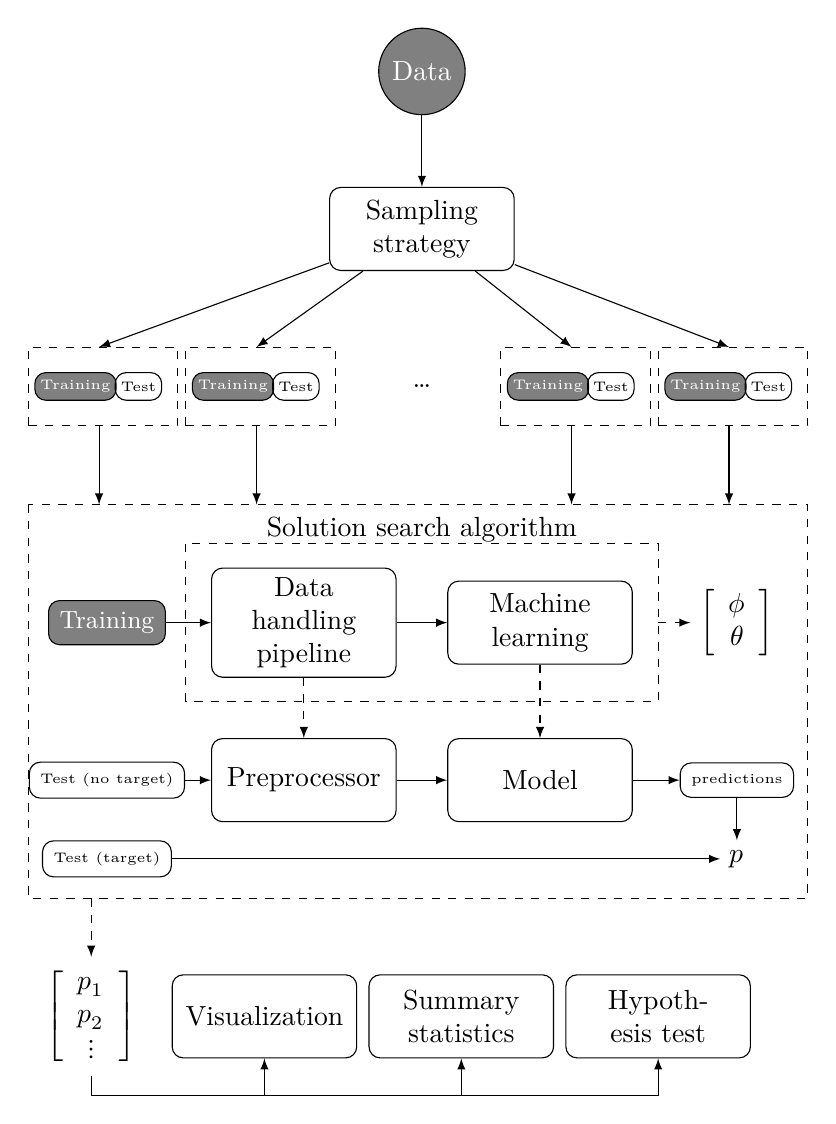
\begin{tikzpicture}
    \node [darkcircle] (data) at (0, 0) {Data};
    \node [block] (sampling) at (0, -2) {Sampling strategy};
    \path [line] (data) -- (sampling);

    \foreach \i in {1, 2, 4, 5} {
      \draw [dashed] (-7 + 2 * \i, -4.5) rectangle (-5.1 + 2 * \i, -3.5);
      \path [line] (sampling) -- (-6.1 + 2 * \i, -3.5);

      \node [smalldarkblock] (train\i) at (-6.4 + 2 * \i, -4) {Training};
      \node [smallblock] (test\i) at (-5.6 + 2 * \i, -4) {Test};

      \path [line] (-6.1 + 2 * \i, -4.5) -- (-6.1 + 2 * \i, -5.5);
    }
    \node [anchor=center] at (0, -4) {\dots};

    \draw [dashed] (-5, -5.5) rectangle (4.9, -10.5);

    \node [smalldarkblock, font=\small, inner sep=4pt] (train) at (-4, -7) {Training};
    \node [smallblock, inner sep=4pt] (test) at (-4, -9) {Test (no target)};

    \draw [dashed] (-3, -6) rectangle (3, -8);
    \node [anchor=south] at (0, -6.1) {Solution search algorithm};

    \node [block] (handling) at (-1.5, -7) {Data handling pipeline};
    \node [block] (learning) at (1.5, -7) {Machine learning};
    \node (model) at (4, -7) {%
      % bracket array with \theta and \phi
      $\left[
      \begin{array}{c}
        \phi \\
        \theta \\
      \end{array}
      \right]$
    };

    \path [line] (train) -- (handling);
    \path [line] (handling) -- (learning);
    \path [line, dashed] (3, -7) -- (model);

    \node [block] (preprocess) at (-1.5, -9) {Preprocessor};
    \node [block] (prediction) at (1.5, -9) {Model};

    \path [line, dashed] (handling) -- (preprocess);
    \path [line, dashed] (learning) -- (prediction);

    \path [line] (test) -- (preprocess);
    \path [line] (preprocess) -- (prediction);

    \node [smallblock, inner sep=4pt] (predicted) at (4, -9) {predictions};
    \node (performance) at (4, -10) {$p$};
    \path [line] (prediction) -- (predicted);

    \node [smallblock, inner sep=4pt] (labels) at (-4, -10) {Test (target)};
    \path [line] (labels) -- (performance);
    \path [line] (predicted) -- (performance);

    \node (perfs) at (-4.2, -12) {%
      $\left[
        \begin{array}{c}
          p_1 \\
          p_2 \\
          \vdots \\
        \end{array}
      \right]$
    };

    \node [block] (visualization) at (-2, -12) {Visualization};
    \node [block] (summary) at (0.5, -12) {Summary statistics};
    \node [block] (hypothesis) at (3, -12) {Hypothesis test};

    \path [line, dashed] (-4.2, -10.5) -- (perfs);
    \path [line] (perfs) -- (-4.2, -13) -- (-2, -13) -- (visualization);
    \path [line] (-2, -13) -- (0.5, -13) -- (summary);
    \path [line] (0.5, -13) -- (3, -13) -- (hypothesis);
  \end{tikzpicture}
  \tcblower
  % A brief description of the experimental plan.
  The experimental plan for estimating the expected performance of a solution involves
  sampling the data, training and testing the solution, evaluating the performance, and
  validating the results.
\end{figurebox}

A summary of the experimental plan for estimating expected performance is shown in
\cref{fig:plan-single}.

\clearpage
\subsection{Cross validation}

The most common sampling strategy is the \emph{cross-validation}.  It assumes that data is
independent and identically distributed (i.i.d.).  The cross-validation technique divides
the dataset into $r$ folds randomly, with the same size.  Each part (fold) is used as a
test set once and as a training set $r-1$ times.  So, first we use as training set folds
$2, 3, \ldots, r$ and as test set fold $1$.  Then, we use as training set folds $1, 3,
\ldots, r$ and as test set fold $2$. And so on.  (See \cref{fig:cross-validation}.)

\begin{figurebox}[label=fig:cross-validation]{Cross-validation}
  \centering
  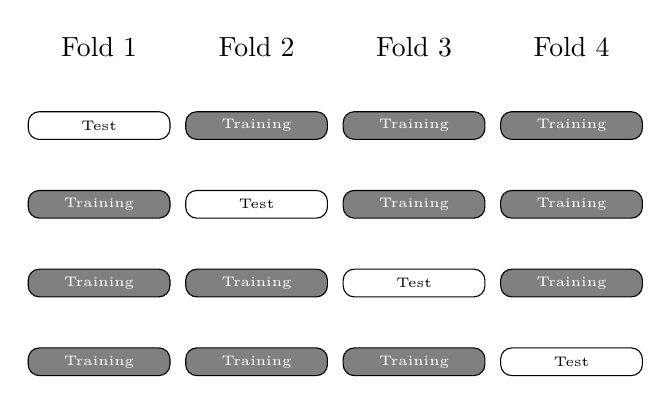
\begin{tikzpicture}
    \foreach \i in {1, 2, 3, 4} {
      \node at (2 * \i, 0) {Fold \i};
      \foreach \j in {1, 2, 3, 4} {
        % if \i == \j, then it is the test set
        \ifnum\i=\j
          \node [smallblock, minimum width=18mm] (fold\i\j) at (2 * \i, -\j) {Test};
        \else
          \node [smalldarkblock, minimum width=18mm] (fold\i\j) at (2 * \i, -\j) {Training};
        \fi
      }
    }
  \end{tikzpicture}
  \tcblower
  Cross-validation is a technique to sample training and test sets.  It divides the
  dataset into $r$ folds, using $r-1$ folds as a training set and the remaining fold as a
  test set.
\end{figurebox}

If possible, one should use repeated
cross-validation, where this process is repeated many times.  Also, when dealing with
classification problems, we should use stratified cross-validation, where the distribution
of the classes is preserved in each fold.

Also, the application of a single cross-validation sampling enables us to create a
predicted vector for the whole dataset.  This is done by concatenating the predictions for
each fold.  (Note however that the predictions are not totally independent, as they share
some training data.  This dependency should be taken into account when analyzing the
results.) This vector can be used to perform hypothesis tests --- like McNemar's test, see
\cref{sub:comparison} --- or to plot ROC (Receiver Operating Characteristic) curves or DET
(Detection Error Tradeoff) curves --- see \cref{chap:evaluation}.

\subsection{Validation methods}

% Talk about summary statistics, visualization (boxplot, roc and det curves), and Bayesian
% analysis.

Validation is the process of interpreting or confirming the meaning of the evaluation
results.  It is the process of determining the degree to which the evaluation results
support the intended use of the solution.

Sometimes, it is as simple as calculating the mean and standard deviation of the
performance samples.  Other times, we need to use more sophisticated techniques, like
hypothesis tests or Bayesian analysis.

Let us say our goal is to reach a certain performance threshold $p_0$.  After an
experiments done with $10$ repeated $10$-fold cross-validation, we have the average
performance $\bar{p}$ and the standard deviation $\sigma$.  If $\bar{p} - \sigma \gg
p_0$, it is very likely that the solution will reach the threshold in production.
Although this is not a formal validation, it is a good and likely enough indication.

Also, it is common to use visualization techniques to analyze the results.  Box plots are
a good way to see the distribution of the performance samples.

A more sophisticated technique is to use Bayesian analysis.  In this case, we use the
performance samples to estimate the probability distribution of the performance of the
algorithm.  This distribution can be used to calculate the probability of the performance
being better than a certain threshold.

\textcite{Benavoli2017} propose an interesting Bayesian test that accounts for the
overlapping training sets in the cross-validation\footnote{%
This is actually a particular case of the proposal in the paper, where the authors
consider the comparison between two performance vector --- which is the case described in
\cref{sub:comparison}.}.
Let $z_k = p_k - p^{*}$ be the
difference between the performance of the $k$-th fold and the performance goal $p^{*}$,
a generative model for the data is
\begin{equation*}
  \vec{z} = \vec{1}\mu + \vec{v}\text{,}
\end{equation*}
where $\vec{z} = (z_1, z_2, \ldots, z_n)$ is the vector performance gains, $\vec{1}$ is a
vector of ones, $\mu$ is the parameter of interest (the mean performance gain), and
$\vec{v} \sim \operatorname{MVN}(0, \Sigma)$ is a multivariate normal noise with zero mean
and covariance matrix $\Sigma$.  The covariance matrix $\Sigma$ is characterized as
\begin{equation*}
  \Sigma_{ii} = \sigma^2\text{,}\quad
  \Sigma_{ij} = \sigma^2\rho\text{,}
\end{equation*}
for all $i \neq j \in \{1, 2, \ldots, n\}$, where $\rho$ is the correlation (between folds)
and $\sigma^2$ is the variance.  The likelihood model of the data is
\begin{equation*}
  \Prob(\vec{z} \mid \mu, \Sigma) =
    \exp\left(-\frac{1}{2}(\vec{z} - \vec{1}\mu)^T \Sigma^{-1} (\vec{z} - \vec{1}\mu)\right)
    \frac{1}{(2\pi)^{n/2} \sqrt{\lvert \Sigma \rvert}}\text{.}
\end{equation*}
According to them, such likelihood does not allow to estimate the correlation from data,
as the maximum likelihood estimate of $\rho$ is zero regardless of the observations.
Since $\rho$ is not identifiable, the authors suggest using the heuristic where $\rho$ is
the ratio between the number of folds and the total number of performance samples.

To estimate the probability of the performance of the solution being greater than the
threshold, we first estimate the parameters $\mu$ and $\nu = \sigma^{-2}$ of the
generative model.  \textcite{Benavoli2017} consider the prior
\begin{equation*}
  \Prob(\mu, \nu \mid \mu_0, \kappa_0, a, b) = \operatorname{NG}(\mu, \nu; \mu_0, \kappa_0, a, b)\text{,}
\end{equation*}
that is a Normal-Gamma distribution with parameters $(\mu_0, \kappa_0, a, b)$.  This is a
conjugate prior to the likelihood model.  Choosing the prior parameters $\mu_0 = 0$,
$\kappa_0 \to \infty$, $a = -1/2$, and $b = 0$, the posterior distribution of $\mu$ is a
location-scale Student distribution.  Mathematically, we have
\begin{equation*}
  \Prob(\mu \mid \vec{z}, \mu_0, \kappa_0, a, b) =
    \operatorname{St}(\mu; n - 1, \bar{z}, \left(
      \frac{1}{n} + \frac{\rho}{1 - \rho}
    \right)s^2)\text{,}
\end{equation*}
where
\begin{equation*}
  \bar{z} = \frac{1}{n} \sum_{i=1}^n z_i\text{,}
\end{equation*}
and
\begin{equation*}
  s^2 = \frac{1}{n - 1} \sum_{i=1}^{n-1} (z_i - \bar{z})^2\text{.}
\end{equation*}

Thus, validating that the solution obtained by the algorithm in production will surpass
the threshold $p^{*}$ consists of calculating the probability
\begin{equation*}
  \Prob(\mu > 0 \mid \vec{z}) > \gamma\text{,}
\end{equation*}
where $\gamma$ is the confidence level.

Note that the Bayesian analysis is a more sophisticated technique than the null hypothesis
significance testing, as it allows us to estimate the probability of the performance of
the solution being better than a certain threshold.

Also, be aware that the choice of the model and the prior distribution can affect the
results.  \textcite{Benavoli2017} suggest using 10 repetitions of 10-fold cross-validation
to estimate the parameters of the generative model.  They also show experimental evidence
that their choices are robust to the choice of the prior distribution.  However, one
should be aware of the limitations of the model.

\section{Comparing strategies}
\label{sub:comparison}

\textcolor{red}{Talk about paired dataset samples.}

When we have two or more strategies to solve a problem, we need to compare them to see
which one is better.  This is a common situation in data science projects, as we usually
have many techniques to solve a problem.

One way to look at this problem is to consider that the algorithm\footnote{That includes
both data handling and machine learning.} $A$ has \emph{hyperparameters} $\lambda \in
\Lambda$.  A hyperparameter here is a parameter that is not learned by the algorithm, but
is set by the user.  For example, the number of neighbors in a k-NN algorithm is a
hyperparameter.  For the sake of generality, we can consider that the hyperparameters may
also include different learning algorithms or data handling pipelines.

Let us say we have a baseline algorithm $A(\lambda_0)$ --- for instance, something that is
in production, the result of the last sprint or a well-known algorithm --- and a new candidate algorithm $A(\lambda)$.
Suppose $\vec{p}(\lambda_0)$ and $\vec{p}(\lambda)$ are the performance vectors of the
baseline and the candidate algorithms, respectively, that are calculated using the same
strategy described in \cref{sec:expected-performance}.  We can validate whether the
candidate is better than the baseline by
\begin{equation*}
  \Prob(\mu > 0 \mid \vec{z}) > \gamma\text{,}
\end{equation*}
where $\vec{z}$ is now $\vec{p}(\lambda) - \vec{p}(\lambda_0)$ and $\gamma$ is the confidence
level.  Also, the expected performance gain of the candidate algorithm is $\mu$ --- if
negative, the performance loss.

This strategy can be applied iteratively to compare many algorithms.  For example, we can
compare $A(\lambda_1)$ with $A(\lambda_0)$, $A(\lambda_2)$ with $A(\lambda_1)$, and so on,
keeping the best algorithm found so far as the baseline. In the cases where the confidence
level is not reached, but the expected performance gain is positive, we can consider
additional characteristics of the algorithms, like the interpretability of the model, the
computational cost, or the ease of implementation, to decide which one is better. However,
one should pay attention whether the probability
\begin{equation*}
  \Prob(\mu < 0 \mid \vec{z})
\end{equation*}
is too high or not.  Always ask yourself if the risk of the performance loss is worth in
the real-world scenario.

\subsection{About nesting experiments}

Mathematically speaking, there is no difference between assessing the choice of
$\left[\phi, \theta\right]$ and the choice of $\lambda$.  Thus, some techniques --- like
grid search --- can be used to find the best hyperparameters using a nested experimental
plan.

The idea is the same, we assess how good is the expected choice of the
hyperparameter-optimization technique $B$ to find the appropriate hyperparameters.  Similarly,
the choice of the hyperparameters and the parameters that goes to production is the
application of $B$ to the whole dataset.  However, never use the choices of the
hyperparameters in the experimental plan to make decisions about what goes to production.
(The same is true for the parameters $\left[\phi, \theta\right]$ in the traditional case.)

\textcolor{red}{We can unnest the search by interpreting the options as different
algorithms two by two.}

\section{Grouping}

TODO Grouped cross validation.

% vim: spell spelllang=en

% \chapter{Ethical, privacy and legal issues}

\chapterprecishere{It's a trap!
  \par\raggedleft--- \textup{Admiral Ackbar}, Star Wars Episode VI: Return of the Jedi}
 TODO

\renewcommand{\theHchapter}{A\arabic{chapter}} % workaround for hyperref
\appendix
\chapter{Preliminaries}
\label{chap:preliminaries}

\chapterprecishere{%
  Maar ik maak steeds wat ik nog niet kan om het te leeren kunnen.\par\raggedleft---
  \textup{Vincent van Gogh}, The Complete Letters of Vincent Van Gogh, Volume Three}

Foundamental concepts in data science come from a variety of fields, including
mathematics, statistics, computer science, optimization theory, and information theory.
This chapter provides a brief overview of the computational, mathematical and statistical
concepts that are used in the rest of the book.

\section{Algorithms and data structures}

Algorithms are step-by-step procedures for solving a problem.  They are used to
manipulate data structures, which are ways of organizing data to solve problems.
They are realized in programming languages, which are formal languages that can be used
to express algorithms.

\subsection{Algoritmic paradigms}

Some techniques are used to solve a wide variety of problems.  They are called
algorithmic paradigms.  The most common ones are listed below.

\paragraph{Divide and conquer}  The problem is divided into smaller subproblems that are
solved recursively.  The solutions to the subproblems are then combined to give a solution
to the original problem.

\paragraph{Dynamic programming}  The problem is divided into overlapping subproblems, and
the solutions to the subproblems are only solved once. The subproblems are then optimized
to find the overall solution.

\paragraph{Greedy algorithms}  The problem is solved with incremental steps, each of which
is locally optimal.  The overall solution is not guaranteed to be optimal.

\subsection{Computational complexity}

Big-O notation, time and space complexity, NP-completeness.

\subsection{Data structures}

Arrays, linked lists, stacks, queues, trees, graphs, hash tables.

\section{Linear algebra}

\subsection{Vectors and matrices}

\subsection{Matrix decompositions}

\textcolor{red}{Verify!}

\paragraph{Singular value decomposition} The singular value decomposition (SVD) of a
matrix $A$ is a factorization of the form
\begin{equation}
  \label{eq:svd}
  A = U \Sigma V^T\text{,}
\end{equation}
where $U$ and $V$ are orthogonal matrices and $\Sigma$ is a diagonal
matrix with non-negative real numbers on the diagonal.  The singular values are the
diagonal entries of $\Sigma$.

\paragraph{Eigenvalue decomposition}  The eigenvalue decomposition of a matrix $A$
is a factorization of the form
\begin{equation}
  \label{eq:eigdec}
  A = Q \Lambda Q^{-1}\text{,}
\end{equation}
where $Q$ is a square matrix whose columns are the eigenvectors of $A$, and
$\Lambda$ is a diagonal matrix whose diagonal entries are the eigenvalues of
$A$.

\paragraph{Cholesky decomposition}  The Cholesky decomposition of a positive-definite
matrix $A$ is a factorization of the form
\begin{equation}
  \label{eq:chol}
  A = L L^T\text{,}
\end{equation}
where $L$ is a lower triangular matrix with real and positive diagonal entries.

\paragraph{QR decomposition}  The QR decomposition of a matrix $A$ is a
factorization of the form
\begin{equation}
  \label{eq:qr}
  A = Q R\text{,}
\end{equation}
where $Q$ is an orthogonal matrix and $R$ is an upper triangular matrix.

\paragraph{LU decomposition}  The LU decomposition of a square matrix $A$ is a
factorization of the form
\begin{equation}
  \label{eq:lu}
  A = L U\text{,}
\end{equation}
where $L$ is a lower triangular matrix with unit diagonal entries and $U$ is
an upper triangular matrix.

\subsection{Eigenvalues and eigenvectors}

An eigenvalue of a square matrix $A$ is a scalar $\lambda$ such that there exists a
non-zero vector $\vec{v}$ satisfying
\begin{equation}
  \label{eq:eig}
  A \vec{v} = \lambda \vec{v}\text{.}
\end{equation}
The vector $\vec{v}$ is called an eigenvector of $A$ corresponding to $\lambda$.

\section{Probability}

\subsection{Axioms of probability}

The Kolmogorov axioms of probability are the foundation of probability theory.
They are
\begin{enumerate}
  \item The probability of an event $E$ is a non-negative real number, i.e. $P(A) \geq 0$;
  \item The probability of the sample space $\Omega$ is one, i.e. $P(\Omega) = 1$; and
  \item The probability of the union of disjoint events, $A \cap B = \emptyset$, is
    the sum of the probabilities of the events, i.e. $P(A \cup B) = P(A) + P(B)$.
\end{enumerate}

\subsection{Permutations and combinations}

\subsection{Conditional probability}

\subsection{Bayes' rule}

\subsection{Independence}

\subsection{Random variables}

\subsection{Probability distributions}

\subsection{Expectation and moments}

\section{Optimization}

\subsection{Minimization of convex functions}

\subsection{Gradient descent}

\subsection{Constraint optimization}

Techniques like Lagrange multipliers, penalty methods, and barrier methods are used to
handle constrained optimization problems in data science.

\subsection{Convex optimization}

Convex optimization problems, where the objective function and the constraints are convex,
have efficient algorithms that guarantee global optimality.

% \subsection{Gradient descent algorithm}
%
% Let $f(\vec{w})$, $f : \mathbb{R}^n \rightarrow \mathbb{R}$, be an objective function that
% we are trying to minimize.  We know that
% $f$ is convex, of class $\mathcal{C}^2$, and its gradient $\nabla f$ is Lipschitz continuous with Lipschitz
% constant $L > 0$.
%
% We want to show that $\lim_{t\rightarrow\infty} f(\vec{w}(t)) = f^{*}$ where $f^{*}$
% is the global minimum of $f$ and $$\vec{w}(t+1) = \vec{w}(t) - \alpha \nabla f(\vec{w}(t))\mbox{,}$$
% for any initial condition $\vec{w}(0)$ and $0 < \alpha \leq \frac{1}{L}$.
%
% Convexity implies that for any two points $\vec{v}$ and $\vec{w}$ in the domain of
% $f$, the line segment connecting them lies above the graph of $f$.  Mathematically, it
% means that $$f(t\vec{v} + (1 - t) \vec{w}) \leq t f(\vec{v}) + (1 - t)
% f(\vec{w})$$ for all $t \in [0, 1]$.
%
% The Lipschitz continuity condition means that the gradient of $f(\vec{w})$ does not change too rapidly.
% Formally, $$\left\|\nabla f(\vec{v}) - \nabla f(\vec{w})\right\| \leq L \|\vec{v} - \vec{w}\|\mbox{,}$$
% for all $\vec{v}$ and $\vec{w}$ in the domain of $f$.  This is a rather weak
% assumption, and it means that the gradient can not change arbitrarily fast.
%
% Since $f$ is convex and twice differentiable, its Hessian is a positive semidefinite
% matrix, and thus its norm is its largest eigenvalue.
%
% A consequence of the Lipschitz continuity for a $\mathcal{C}^2$ function $f$ is that for
% any $\vec{v}$ and $\vec{w}$, we have that
% \begin{equation}
%   \label{eq:lcg1}
%   \vec{v}^T \nabla^2 f(w) \vec{v} \leq L \|v\|^2\text{.}
% \end{equation}
% It means that the eigenvalues of the Hessian are bounded above by $L$.
%
% \paragraph{Descent lemma.}  For $f$, a the multivariate Taylor expansion is that
% $$f(w) = f(v)$$

\input{machines}

\backmatter
\printbibliography
\printglossary

\end{document}
